% Options for packages loaded elsewhere
\PassOptionsToPackage{unicode}{hyperref}
\PassOptionsToPackage{hyphens}{url}
%
\documentclass[
]{article}
\usepackage{amsmath,amssymb}
\usepackage{iftex}
\ifPDFTeX
  \usepackage[T1]{fontenc}
  \usepackage[utf8]{inputenc}
  \usepackage{textcomp} % provide euro and other symbols
\else % if luatex or xetex
  \usepackage{unicode-math} % this also loads fontspec
  \defaultfontfeatures{Scale=MatchLowercase}
  \defaultfontfeatures[\rmfamily]{Ligatures=TeX,Scale=1}
\fi
\usepackage{lmodern}
\ifPDFTeX\else
  % xetex/luatex font selection
\fi
% Use upquote if available, for straight quotes in verbatim environments
\IfFileExists{upquote.sty}{\usepackage{upquote}}{}
\IfFileExists{microtype.sty}{% use microtype if available
  \usepackage[]{microtype}
  \UseMicrotypeSet[protrusion]{basicmath} % disable protrusion for tt fonts
}{}
\makeatletter
\@ifundefined{KOMAClassName}{% if non-KOMA class
  \IfFileExists{parskip.sty}{%
    \usepackage{parskip}
  }{% else
    \setlength{\parindent}{0pt}
    \setlength{\parskip}{6pt plus 2pt minus 1pt}}
}{% if KOMA class
  \KOMAoptions{parskip=half}}
\makeatother
\usepackage{xcolor}
\usepackage[margin=1in]{geometry}
\usepackage{color}
\usepackage{fancyvrb}
\newcommand{\VerbBar}{|}
\newcommand{\VERB}{\Verb[commandchars=\\\{\}]}
\DefineVerbatimEnvironment{Highlighting}{Verbatim}{commandchars=\\\{\}}
% Add ',fontsize=\small' for more characters per line
\usepackage{framed}
\definecolor{shadecolor}{RGB}{248,248,248}
\newenvironment{Shaded}{\begin{snugshade}}{\end{snugshade}}
\newcommand{\AlertTok}[1]{\textcolor[rgb]{0.94,0.16,0.16}{#1}}
\newcommand{\AnnotationTok}[1]{\textcolor[rgb]{0.56,0.35,0.01}{\textbf{\textit{#1}}}}
\newcommand{\AttributeTok}[1]{\textcolor[rgb]{0.13,0.29,0.53}{#1}}
\newcommand{\BaseNTok}[1]{\textcolor[rgb]{0.00,0.00,0.81}{#1}}
\newcommand{\BuiltInTok}[1]{#1}
\newcommand{\CharTok}[1]{\textcolor[rgb]{0.31,0.60,0.02}{#1}}
\newcommand{\CommentTok}[1]{\textcolor[rgb]{0.56,0.35,0.01}{\textit{#1}}}
\newcommand{\CommentVarTok}[1]{\textcolor[rgb]{0.56,0.35,0.01}{\textbf{\textit{#1}}}}
\newcommand{\ConstantTok}[1]{\textcolor[rgb]{0.56,0.35,0.01}{#1}}
\newcommand{\ControlFlowTok}[1]{\textcolor[rgb]{0.13,0.29,0.53}{\textbf{#1}}}
\newcommand{\DataTypeTok}[1]{\textcolor[rgb]{0.13,0.29,0.53}{#1}}
\newcommand{\DecValTok}[1]{\textcolor[rgb]{0.00,0.00,0.81}{#1}}
\newcommand{\DocumentationTok}[1]{\textcolor[rgb]{0.56,0.35,0.01}{\textbf{\textit{#1}}}}
\newcommand{\ErrorTok}[1]{\textcolor[rgb]{0.64,0.00,0.00}{\textbf{#1}}}
\newcommand{\ExtensionTok}[1]{#1}
\newcommand{\FloatTok}[1]{\textcolor[rgb]{0.00,0.00,0.81}{#1}}
\newcommand{\FunctionTok}[1]{\textcolor[rgb]{0.13,0.29,0.53}{\textbf{#1}}}
\newcommand{\ImportTok}[1]{#1}
\newcommand{\InformationTok}[1]{\textcolor[rgb]{0.56,0.35,0.01}{\textbf{\textit{#1}}}}
\newcommand{\KeywordTok}[1]{\textcolor[rgb]{0.13,0.29,0.53}{\textbf{#1}}}
\newcommand{\NormalTok}[1]{#1}
\newcommand{\OperatorTok}[1]{\textcolor[rgb]{0.81,0.36,0.00}{\textbf{#1}}}
\newcommand{\OtherTok}[1]{\textcolor[rgb]{0.56,0.35,0.01}{#1}}
\newcommand{\PreprocessorTok}[1]{\textcolor[rgb]{0.56,0.35,0.01}{\textit{#1}}}
\newcommand{\RegionMarkerTok}[1]{#1}
\newcommand{\SpecialCharTok}[1]{\textcolor[rgb]{0.81,0.36,0.00}{\textbf{#1}}}
\newcommand{\SpecialStringTok}[1]{\textcolor[rgb]{0.31,0.60,0.02}{#1}}
\newcommand{\StringTok}[1]{\textcolor[rgb]{0.31,0.60,0.02}{#1}}
\newcommand{\VariableTok}[1]{\textcolor[rgb]{0.00,0.00,0.00}{#1}}
\newcommand{\VerbatimStringTok}[1]{\textcolor[rgb]{0.31,0.60,0.02}{#1}}
\newcommand{\WarningTok}[1]{\textcolor[rgb]{0.56,0.35,0.01}{\textbf{\textit{#1}}}}
\usepackage{graphicx}
\makeatletter
\def\maxwidth{\ifdim\Gin@nat@width>\linewidth\linewidth\else\Gin@nat@width\fi}
\def\maxheight{\ifdim\Gin@nat@height>\textheight\textheight\else\Gin@nat@height\fi}
\makeatother
% Scale images if necessary, so that they will not overflow the page
% margins by default, and it is still possible to overwrite the defaults
% using explicit options in \includegraphics[width, height, ...]{}
\setkeys{Gin}{width=\maxwidth,height=\maxheight,keepaspectratio}
% Set default figure placement to htbp
\makeatletter
\def\fps@figure{htbp}
\makeatother
\setlength{\emergencystretch}{3em} % prevent overfull lines
\providecommand{\tightlist}{%
  \setlength{\itemsep}{0pt}\setlength{\parskip}{0pt}}
\setcounter{secnumdepth}{-\maxdimen} % remove section numbering
\ifLuaTeX
  \usepackage{selnolig}  % disable illegal ligatures
\fi
\IfFileExists{bookmark.sty}{\usepackage{bookmark}}{\usepackage{hyperref}}
\IfFileExists{xurl.sty}{\usepackage{xurl}}{} % add URL line breaks if available
\urlstyle{same}
\hypersetup{
  pdftitle={ACRM 2023 Longitudinal Data Analysis Workshop},
  pdfauthor={Keith Lohse, PhD, PStat, and Allan Kozlowski, PhD, BsC (PT)},
  hidelinks,
  pdfcreator={LaTeX via pandoc}}

\title{ACRM 2023 Longitudinal Data Analysis Workshop}
\author{Keith Lohse, PhD, PStat, and Allan Kozlowski, PhD, BsC (PT)}
\date{}

\begin{document}
\maketitle

\hypertarget{practical-session-4-simulation-based-approaches-to-statistical-power-in-mixed-effect-models}{%
\section{Practical Session 4: Simulation-based Approaches to Statistical
Power in Mixed-Effect
Models}\label{practical-session-4-simulation-based-approaches-to-statistical-power-in-mixed-effect-models}}

\hypertarget{a-refresher-about-statistical-power}{%
\subsection{1.A Refresher about Statistical
Power}\label{a-refresher-about-statistical-power}}

In previous sessions, we explored how to visualize longitudinal data,
how to build mixed-effect regression models, and how to conduct
statistical significance tests in the context of linear and non-linear
mixed-effect regression. In this session, we will focus on statistical
power as a complement to null-hypothesis testing.

As before, we will use several packages related to data management,
visualization, and mixed-effect models.

\begin{Shaded}
\begin{Highlighting}[]
\CommentTok{\# Loading the essential libraries. }
\FunctionTok{library}\NormalTok{(}\StringTok{"tidyverse"}\NormalTok{); }\FunctionTok{library}\NormalTok{(}\StringTok{"lme4"}\NormalTok{); }\FunctionTok{library}\NormalTok{(}\StringTok{"MASS"}\NormalTok{)}
\FunctionTok{library}\NormalTok{(}\StringTok{"car"}\NormalTok{); }\FunctionTok{library}\NormalTok{(}\StringTok{"lmerTest"}\NormalTok{);}\FunctionTok{library}\NormalTok{(}\StringTok{"nlme"}\NormalTok{); }\FunctionTok{library}\NormalTok{(}\StringTok{"patchwork"}\NormalTok{)}
\end{Highlighting}
\end{Shaded}

If you have not already installed these packages, you will need to use
the install.packages() function first. This can take some time and will
require an internet connection.

\begin{Shaded}
\begin{Highlighting}[]
\CommentTok{\# If these packages are not installed already, run the following code: }
\FunctionTok{install.packages}\NormalTok{(}\StringTok{"tidyverse"}\NormalTok{); }\FunctionTok{install.packages}\NormalTok{(}\StringTok{"lme4"}\NormalTok{); }
\FunctionTok{install.packages}\NormalTok{(}\StringTok{"car"}\NormalTok{); }\FunctionTok{install.packages}\NormalTok{(}\StringTok{"lmerTest"}\NormalTok{); }\FunctionTok{install.packages}\NormalTok{(}\StringTok{"nlme"}\NormalTok{)}
\end{Highlighting}
\end{Shaded}

Before we get into the details of hypothesis testing with longitudinal
data, let's briefly refresh the concept of statistical power.
Calculating statistical power requires us to first figure out what would
happen under the \emph{null hypothesis}. In this case we assume that the
true mean difference is zero (H0: \(\delta\)=0). If the null hypothesis
were true, we would expect a distribution of mean differences like the
one in blue. The distribution is centered on 0, but the difference we
observe will vary from study to study. Specifically, 95\% of the null
distribution is between the vertical black lines, putting 2.5\% in each
tail. If a mean difference falls outside of those black lines (i.e.,
p\textless0.05 if the null is true), then we would call the result
``statistically significant'' and reject the null hypothesis. We use
\(\alpha\)=0.05 as a cutoff by convention, but this limit could be set
to any value and conventions will vary by scientific discipline.
Critically though, by setting this \(\alpha\) threshold allows us to
control the Type I error rate. That is, if we set \(\alpha\)=0.05, that
means we will only make a mistake and declare an effect statistically
significant 5\% time when the null is true (i.e., we will make ``false
alarms'' 5\% of the time).

However, we also need to consider what might happen if the null is
\emph{not} true. For instance, what if the true mean difference was
\(\delta\)=4 instead of \(\delta\)=0? If this \emph{alternative
hypothesis} was true, then we would expect a distribution of mean
differences like the one in red. Under this assumption, 50\% of our
results are above the statistical significance threshold and 50\% are
below the threshold. Thus, if \(\delta\)=4 is true, we will fail to find
a statistically significant effect 50\% of the time (i.e., we will miss
50\% of the time). This miss rate is referred to as the Type II error
rate and represented by \(\beta\).

Statistical power is 1-\(\beta\). Put another way, statistical power is
the probability of obtaining a statistically significant result if a
given alternative hypothesis is true. In the figure, statistical power
is not very good, because if the true mean difference is \(\delta\)=4,
we will only correctly reject the null hypothesis 50\% of the time!

\begin{Shaded}
\begin{Highlighting}[]
\NormalTok{differences }\OtherTok{\textless{}{-}} \FunctionTok{c}\NormalTok{(}\FunctionTok{seq}\NormalTok{(}\SpecialCharTok{{-}}\DecValTok{10}\NormalTok{, }\DecValTok{10}\NormalTok{, }\FloatTok{0.1}\NormalTok{))}
\NormalTok{null\_dist }\OtherTok{\textless{}{-}} \FunctionTok{dnorm}\NormalTok{(}\AttributeTok{x=}\NormalTok{differences, }\AttributeTok{mean=}\DecValTok{0}\NormalTok{, }\AttributeTok{sd=}\DecValTok{2}\NormalTok{)}
\NormalTok{alt\_dist }\OtherTok{\textless{}{-}} \FunctionTok{dnorm}\NormalTok{(}\AttributeTok{x=}\NormalTok{differences, }\AttributeTok{mean=}\DecValTok{4}\NormalTok{, }\AttributeTok{sd=}\DecValTok{2}\NormalTok{)}

\NormalTok{DATA }\OtherTok{\textless{}{-}} \FunctionTok{data.frame}\NormalTok{(differences, null\_dist, alt\_dist)}
\end{Highlighting}
\end{Shaded}

\begin{Shaded}
\begin{Highlighting}[]
\NormalTok{cbPalette }\OtherTok{\textless{}{-}} \FunctionTok{c}\NormalTok{(}\StringTok{"\#999999"}\NormalTok{, }\StringTok{"\#E69F00"}\NormalTok{, }\StringTok{"\#56B4E9"}\NormalTok{, }\StringTok{"\#009E73"}\NormalTok{, }\StringTok{"\#CC79A7"}\NormalTok{, }\StringTok{"\#F0E442"}\NormalTok{,  }
               \StringTok{"\#555555"}\NormalTok{,  }\StringTok{"\#D55E00"}\NormalTok{,}\StringTok{"\#0072B2"}\NormalTok{, }\StringTok{"\#03c478"}\NormalTok{, }\StringTok{"\#661100"}\NormalTok{, }\StringTok{"\#f3f319"}\NormalTok{,  }
               \StringTok{"\#222222"}\NormalTok{,}\StringTok{"\#FBD7A2"}\NormalTok{, }\StringTok{"\#6699CC"}\NormalTok{, }\StringTok{"\#99edcc"}\NormalTok{, }\StringTok{"\#b804a2"}\NormalTok{, }\StringTok{"\#F9E999"}\NormalTok{)}

\FunctionTok{ggplot}\NormalTok{(}\AttributeTok{data=}\NormalTok{DATA, }\FunctionTok{aes}\NormalTok{(}\AttributeTok{x=}\NormalTok{differences)) }\SpecialCharTok{+}
  \FunctionTok{geom\_density}\NormalTok{(}\FunctionTok{aes}\NormalTok{(}\AttributeTok{y=}\NormalTok{null\_dist), }\AttributeTok{fill=}\NormalTok{cbPalette[}\DecValTok{3}\NormalTok{], }\AttributeTok{stat=}\StringTok{"identity"}\NormalTok{, }\AttributeTok{alpha=}\FloatTok{0.5}\NormalTok{)}\SpecialCharTok{+}
  \FunctionTok{geom\_density}\NormalTok{(}\FunctionTok{aes}\NormalTok{(}\AttributeTok{y=}\NormalTok{alt\_dist), }\AttributeTok{fill=}\NormalTok{cbPalette[}\DecValTok{5}\NormalTok{], }\AttributeTok{stat=}\StringTok{"identity"}\NormalTok{, }\AttributeTok{alpha=}\FloatTok{0.5}\NormalTok{)}\SpecialCharTok{+}
  \FunctionTok{geom\_vline}\NormalTok{(}\AttributeTok{xintercept =} \FunctionTok{c}\NormalTok{(}\SpecialCharTok{{-}}\DecValTok{4}\NormalTok{, }\DecValTok{4}\NormalTok{), }\AttributeTok{lty=}\DecValTok{2}\NormalTok{, }\AttributeTok{lwd=}\DecValTok{1}\NormalTok{, }\AttributeTok{col=}\StringTok{"black"}\NormalTok{)}\SpecialCharTok{+}
  \FunctionTok{scale\_x\_continuous}\NormalTok{(}\AttributeTok{name =} \FunctionTok{expression}\NormalTok{(delta)) }\SpecialCharTok{+}
  \FunctionTok{scale\_y\_continuous}\NormalTok{(}\AttributeTok{name =} \StringTok{"Density"}\NormalTok{) }\SpecialCharTok{+}
  \FunctionTok{theme\_bw}\NormalTok{()}\SpecialCharTok{+}
  \FunctionTok{theme}\NormalTok{(}\AttributeTok{axis.text=}\FunctionTok{element\_text}\NormalTok{(}\AttributeTok{size=}\DecValTok{10}\NormalTok{, }\AttributeTok{color=}\StringTok{"black"}\NormalTok{),}
        \AttributeTok{legend.text=}\FunctionTok{element\_text}\NormalTok{(}\AttributeTok{size=}\DecValTok{10}\NormalTok{, }\AttributeTok{color=}\StringTok{"black"}\NormalTok{),}
        \AttributeTok{legend.title=}\FunctionTok{element\_text}\NormalTok{(}\AttributeTok{size=}\DecValTok{10}\NormalTok{, }\AttributeTok{face=}\StringTok{"bold"}\NormalTok{),}
        \AttributeTok{axis.title=}\FunctionTok{element\_text}\NormalTok{(}\AttributeTok{size=}\DecValTok{12}\NormalTok{, }\AttributeTok{face=}\StringTok{"bold"}\NormalTok{),}
        \AttributeTok{plot.title=}\FunctionTok{element\_text}\NormalTok{(}\AttributeTok{size=}\DecValTok{12}\NormalTok{, }\AttributeTok{face=}\StringTok{"bold"}\NormalTok{, }\AttributeTok{hjust=}\FloatTok{0.5}\NormalTok{),}
        \AttributeTok{panel.grid.minor =} \FunctionTok{element\_blank}\NormalTok{(),}
        \AttributeTok{strip.text =} \FunctionTok{element\_text}\NormalTok{(}\AttributeTok{size=}\DecValTok{10}\NormalTok{, }\AttributeTok{face=}\StringTok{"bold"}\NormalTok{),}
        \AttributeTok{legend.position =} \StringTok{"none"}\NormalTok{)}
\end{Highlighting}
\end{Shaded}

\begin{center}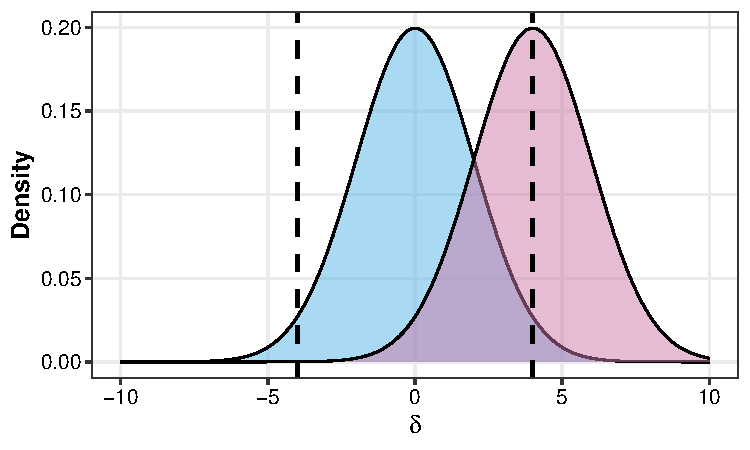
\includegraphics{lohse_ACRM_2023_module_04_files/figure-latex/figure 1-1} \end{center}

This figure highlights why we can't solely focus on getting
statistically significant results. The alternative hypothesis might very
well be true, but if we do not have enough people/observations, then we
may lack the statistical power to detect it. Thus, anytime you are
designing a study you need to consider statistical power, how high you
want statistical power to be, and what changes you might be able to make
to improve statistical power. E.g.,

\begin{enumerate}
\def\labelenumi{\arabic{enumi}.}
\tightlist
\item
  Increasing the size of the effect (e.g., giving a drug at a high dose
  compared to a moderate dose).
\item
  Reducing the variability in the data (e.g., through
  inclusion/exclusion criteria or controlling for relevant covariates).
\item
  Increasing the number of observations (e.g., recruiting more
  participants and/or taking more observations per participant)
\end{enumerate}

In the context of longitudinal studies, we are commonly most interested
in \emph{cross-level interactions}. For instance, did people receiving
the experimental treatment change at the same rate as people receiving
the control treatment? Or, do people with more severe baseline
impairment show similar trajectories compared to people with less severe
baseline impairment? These Group x Time interactions can take many forms
and we cannot possibly cover them all here. However, we will try to
provide some fundamental tools and show the logic of using simulation
based approaches to statistical power. Users can then adapt this code to
their specific case, changing things like the number of observations,
the amount and pattern of missing data, the (non)linearity of their
trajectories, and the magnitude of the effects they are predicting.

\hypertarget{a-simulation-approach-to-longitudinal-data}{%
\section{2. A Simulation Approach to Longitudinal
Data}\label{a-simulation-approach-to-longitudinal-data}}

There are many tools that provide \emph{analytical} solutions to
statistical power in mixed models (e.g.,
\url{https://glimmpse.samplesizeshop.org/};
\url{https://jakewestfall.shinyapps.io/pangea/}). However, I think the
simulation approach is very useful because it allows users to generate
\emph{empirical} solutions for very complex cases that are not easily
accounted for by analytical packages (e.g., unequal spacing of time
points, different types of missing data, differing random effects). The
mathematics of mixed-effect regression are very complex and there is not
always complete agreement on \emph{how} effects should be estimated or
if p-values should even be calculated (see:
\url{https://stat.ethz.ch/pipermail/r-help/2006-May/094765.html}).
Obviously, this makes a formal calculation of statistical power
difficult, as you cannot confidently test p\textless0.05 if not everyone
agrees on how p should be calculated.

Far from being impossible however, I would encourage you to think about
statistical power in mixed-models as ``squishy''. For instance,
flexibility in the structure of the random effects or choices in the
methods of estimation can lead to different p-values. However, there are
definitely some \emph{incorrect} approaches (e.g., under-specified or
mis-specified random effects) and being able to simulate your own data
then allows you to test the effect of your different modelling choices
on the outcome.

In this section, we will simulate a relatively simple longitudinal data
structure with 4-5 observations for 10 individuals. The data are missing
at random with the exception of every participant having the first
observation. In the code chunk below, we set the number of individuals,
the values for the fixed effects, and the values for the random effects.

\begin{Shaded}
\begin{Highlighting}[]
\NormalTok{N }\OtherTok{\textless{}{-}} \DecValTok{10} \CommentTok{\# set number of individuals}

\CommentTok{\# Fixed Effects}
\NormalTok{beta0 }\OtherTok{\textless{}{-}} \FloatTok{50.0} \CommentTok{\# population intercept }
\NormalTok{beta1 }\OtherTok{\textless{}{-}} \FloatTok{1.0}  \CommentTok{\# population slope}

\CommentTok{\# Random Effects and Errors}
\NormalTok{tau0  }\OtherTok{\textless{}{-}} \DecValTok{10} \CommentTok{\# intercept SD, }
\NormalTok{tau1  }\OtherTok{\textless{}{-}} \FloatTok{2.0} \CommentTok{\# slope SD, }
\NormalTok{tau01 }\OtherTok{\textless{}{-}} \FloatTok{0.5} \CommentTok{\# correlation between slope and intercept,}
\NormalTok{sigma }\OtherTok{\textless{}{-}} \DecValTok{5} \CommentTok{\# true error SD}


\CommentTok{\# number of possible observations per person}
\NormalTok{max\_obs }\OtherTok{\textless{}{-}} \DecValTok{5}
\NormalTok{min\_obs }\OtherTok{\textless{}{-}} \DecValTok{4}
\end{Highlighting}
\end{Shaded}

With these starting values in place, we can simulate a random number of
observations per person, constrained to between the minimum and maximum
number of observations we set above. Finally, we bind the subject
identifiers together with the time variable into a dataframe called
\emph{DATA}. The first six rows of the dataframe are shown.

\begin{Shaded}
\begin{Highlighting}[]
\CommentTok{\# simulate MISSING AT RANDOM observations for each individual}
\FunctionTok{set.seed}\NormalTok{(}\DecValTok{42}\NormalTok{)}
\NormalTok{p }\OtherTok{\textless{}{-}} \FunctionTok{round}\NormalTok{(}\FunctionTok{runif}\NormalTok{(}\AttributeTok{n=}\NormalTok{N, }\AttributeTok{min=}\NormalTok{min\_obs, }\AttributeTok{max=}\NormalTok{max\_obs))}

\CommentTok{\# simulate observations per person (everyone has 1st observation)}
\NormalTok{time }\OtherTok{\textless{}{-}} \FunctionTok{unlist}\NormalTok{(}\FunctionTok{sapply}\NormalTok{(p, }\ControlFlowTok{function}\NormalTok{(x) }\FunctionTok{c}\NormalTok{(}\DecValTok{1}\NormalTok{, }\FunctionTok{sort}\NormalTok{(}\FunctionTok{sample}\NormalTok{(}\AttributeTok{x=}\DecValTok{2}\SpecialCharTok{:}\NormalTok{max\_obs, }\AttributeTok{size =}\NormalTok{ x}\DecValTok{{-}1}\NormalTok{, }\AttributeTok{replace=}\ConstantTok{FALSE}\NormalTok{)))))}

\CommentTok{\# set up data frame}
\NormalTok{DATA }\OtherTok{\textless{}{-}} \FunctionTok{data.frame}\NormalTok{(}\AttributeTok{id=}\FunctionTok{rep}\NormalTok{(}\DecValTok{1}\SpecialCharTok{:}\NormalTok{N, }\AttributeTok{times=}\NormalTok{p), }\AttributeTok{time=}\NormalTok{time)}

\FunctionTok{head}\NormalTok{(DATA)}
\end{Highlighting}
\end{Shaded}

\begin{verbatim}
##   id time
## 1  1    1
## 2  1    2
## 3  1    3
## 4  1    4
## 5  1    5
## 6  2    1
\end{verbatim}

Next, we will create the actual data. To do this, we will take the
scalar variance and covariance values that we set above, and then use
those values to obtain correlated random effects.

\begin{Shaded}
\begin{Highlighting}[]
\NormalTok{mu  }\OtherTok{\textless{}{-}} \FunctionTok{c}\NormalTok{(}\DecValTok{0}\NormalTok{,}\DecValTok{0}\NormalTok{) }\CommentTok{\# random effects are assumed to be normally distributed with a mean of 0}
\NormalTok{S   }\OtherTok{\textless{}{-}} \FunctionTok{matrix}\NormalTok{(}\FunctionTok{c}\NormalTok{(}\DecValTok{1}\NormalTok{, tau01, tau01, }\DecValTok{1}\NormalTok{), }\AttributeTok{nrow=}\DecValTok{2}\NormalTok{) }\CommentTok{\# correlation matrix for the randomw slope and intercept}
\NormalTok{taus }\OtherTok{\textless{}{-}} \FunctionTok{c}\NormalTok{(tau0, tau1) }\CommentTok{\# vector of random effect variances}
\NormalTok{S   }\OtherTok{\textless{}{-}} \FunctionTok{diag}\NormalTok{(taus) }\SpecialCharTok{\%*\%}\NormalTok{ S }\SpecialCharTok{\%*\%} \FunctionTok{diag}\NormalTok{(taus) }\CommentTok{\# rescaling our correlation matrix to be a covariance matrix}
\NormalTok{U   }\OtherTok{\textless{}{-}} \FunctionTok{mvrnorm}\NormalTok{(N, }\AttributeTok{mu=}\NormalTok{mu, }\AttributeTok{Sigma=}\NormalTok{S) }\CommentTok{\# Creating random deviates for the random slope and intercept, equal to length N, and means mu and variances S.}
\end{Highlighting}
\end{Shaded}

Next, at the level of individual observations, we will simulate random
errors. Note you could also simulate correlated residuals in this step,
but this is an advanced topic. For the moment, we will assume that these
errors are independent of each other with a mean = 0 and a standard
deviation equal to \(sigma\) that we defined above.

\begin{Shaded}
\begin{Highlighting}[]
\CommentTok{\# simulate (uncorrelated) residuals}
\CommentTok{\# you could instead simulate correlated residuals, but that takes a bit more work}
\FunctionTok{set.seed}\NormalTok{(}\DecValTok{42}\NormalTok{)}
\NormalTok{DATA}\SpecialCharTok{$}\NormalTok{eij }\OtherTok{\textless{}{-}} \FunctionTok{rnorm}\NormalTok{(}\AttributeTok{n=}\FunctionTok{nrow}\NormalTok{(DATA), }\AttributeTok{mean=}\DecValTok{0}\NormalTok{, }\AttributeTok{sd=}\NormalTok{sigma)}

\FunctionTok{head}\NormalTok{(DATA)}
\end{Highlighting}
\end{Shaded}

\begin{verbatim}
##   id time        eij
## 1  1    1  6.8547922
## 2  1    2 -2.8234909
## 3  1    3  1.8156421
## 4  1    4  3.1643130
## 5  1    5  2.0213416
## 6  2    1 -0.5306226
\end{verbatim}

Finally, we can combine the fixed effects, the random deviates (for each
participant), and the random errors (for each observation) to simulate
longitudinal data with time nested within participants. We will print
the first six rows of the data and then generate a plot showing all of
the data for these 10 participants.

\begin{Shaded}
\begin{Highlighting}[]
\NormalTok{DATA}\SpecialCharTok{$}\NormalTok{yij }\OtherTok{\textless{}{-}}\NormalTok{ (beta0 }\SpecialCharTok{+} \FunctionTok{rep}\NormalTok{(U[,}\DecValTok{1}\NormalTok{], }\AttributeTok{times=}\NormalTok{p)) }\SpecialCharTok{+} 
\NormalTok{  (beta1 }\SpecialCharTok{+} \FunctionTok{rep}\NormalTok{(U[,}\DecValTok{2}\NormalTok{], }\AttributeTok{times=}\NormalTok{p)) }\SpecialCharTok{*}\NormalTok{ DATA}\SpecialCharTok{$}\NormalTok{time }\SpecialCharTok{+}\NormalTok{ DATA}\SpecialCharTok{$}\NormalTok{eij}

\FunctionTok{head}\NormalTok{(DATA)}
\end{Highlighting}
\end{Shaded}

\begin{verbatim}
##   id time        eij      yij
## 1  1    1  6.8547922 65.24221
## 2  1    2 -2.8234909 59.95065
## 3  1    3  1.8156421 68.97651
## 4  1    4  3.1643130 74.71190
## 5  1    5  2.0213416 77.95566
## 6  2    1 -0.5306226 54.51284
\end{verbatim}

\begin{Shaded}
\begin{Highlighting}[]
\NormalTok{cbPalette }\OtherTok{\textless{}{-}} \FunctionTok{c}\NormalTok{(}\StringTok{"\#999999"}\NormalTok{, }\StringTok{"\#E69F00"}\NormalTok{, }\StringTok{"\#56B4E9"}\NormalTok{, }\StringTok{"\#009E73"}\NormalTok{, }\StringTok{"\#CC79A7"}\NormalTok{, }\StringTok{"\#F0E442"}\NormalTok{,  }
               \StringTok{"\#555555"}\NormalTok{,  }\StringTok{"\#D55E00"}\NormalTok{,}\StringTok{"\#0072B2"}\NormalTok{, }\StringTok{"\#03c478"}\NormalTok{, }\StringTok{"\#661100"}\NormalTok{, }\StringTok{"\#f3f319"}\NormalTok{,  }
               \StringTok{"\#222222"}\NormalTok{,}\StringTok{"\#FBD7A2"}\NormalTok{, }\StringTok{"\#6699CC"}\NormalTok{, }\StringTok{"\#99edcc"}\NormalTok{, }\StringTok{"\#b804a2"}\NormalTok{, }\StringTok{"\#F9E999"}\NormalTok{)}

\CommentTok{\# Lattice plot of the example data {-}{-}{-}{-}}
\FunctionTok{ggplot}\NormalTok{(}\AttributeTok{data=}\NormalTok{DATA, }\FunctionTok{aes}\NormalTok{(}\AttributeTok{x=}\NormalTok{time, }\AttributeTok{y=}\NormalTok{yij)) }\SpecialCharTok{+}
  \FunctionTok{geom\_point}\NormalTok{(}\AttributeTok{shape=}\DecValTok{16}\NormalTok{, }\AttributeTok{col=}\StringTok{"black"}\NormalTok{)}\SpecialCharTok{+}
  \FunctionTok{geom\_line}\NormalTok{(}\AttributeTok{col=}\StringTok{"black"}\NormalTok{)}\SpecialCharTok{+}
  \FunctionTok{stat\_smooth}\NormalTok{(}\FunctionTok{aes}\NormalTok{(}\AttributeTok{group=}\NormalTok{id), }\AttributeTok{col=}\StringTok{"blue"}\NormalTok{, }\AttributeTok{se=}\ConstantTok{FALSE}\NormalTok{, }
              \AttributeTok{method=}\StringTok{"lm"}\NormalTok{)}\SpecialCharTok{+}
  \FunctionTok{scale\_x\_continuous}\NormalTok{(}\AttributeTok{name =} \StringTok{"Time"}\NormalTok{) }\SpecialCharTok{+}
  \FunctionTok{scale\_y\_continuous}\NormalTok{(}\AttributeTok{name =} \StringTok{"Outcome"}\NormalTok{) }\SpecialCharTok{+}
  \FunctionTok{facet\_wrap}\NormalTok{(}\SpecialCharTok{\textasciitilde{}}\NormalTok{id, }\AttributeTok{ncol=}\DecValTok{5}\NormalTok{) }\SpecialCharTok{+}
  \FunctionTok{theme\_bw}\NormalTok{()}\SpecialCharTok{+}
  \FunctionTok{theme}\NormalTok{(}\AttributeTok{axis.text=}\FunctionTok{element\_text}\NormalTok{(}\AttributeTok{size=}\DecValTok{10}\NormalTok{, }\AttributeTok{color=}\StringTok{"black"}\NormalTok{),}
        \AttributeTok{legend.text=}\FunctionTok{element\_text}\NormalTok{(}\AttributeTok{size=}\DecValTok{10}\NormalTok{, }\AttributeTok{color=}\StringTok{"black"}\NormalTok{),}
        \AttributeTok{legend.title=}\FunctionTok{element\_text}\NormalTok{(}\AttributeTok{size=}\DecValTok{10}\NormalTok{, }\AttributeTok{face=}\StringTok{"bold"}\NormalTok{),}
        \AttributeTok{axis.title=}\FunctionTok{element\_text}\NormalTok{(}\AttributeTok{size=}\DecValTok{10}\NormalTok{, }\AttributeTok{face=}\StringTok{"bold"}\NormalTok{),}
        \AttributeTok{plot.title=}\FunctionTok{element\_text}\NormalTok{(}\AttributeTok{size=}\DecValTok{12}\NormalTok{, }\AttributeTok{face=}\StringTok{"bold"}\NormalTok{, }\AttributeTok{hjust=}\FloatTok{0.5}\NormalTok{),}
        \AttributeTok{panel.grid.minor =} \FunctionTok{element\_blank}\NormalTok{(),}
        \AttributeTok{strip.text =} \FunctionTok{element\_text}\NormalTok{(}\AttributeTok{size=}\DecValTok{10}\NormalTok{, }\AttributeTok{face=}\StringTok{"bold"}\NormalTok{),}
        \AttributeTok{legend.position =} \StringTok{"none"}\NormalTok{)}
\end{Highlighting}
\end{Shaded}

\begin{verbatim}
## `geom_smooth()` using formula 'y ~ x'
\end{verbatim}

\begin{center}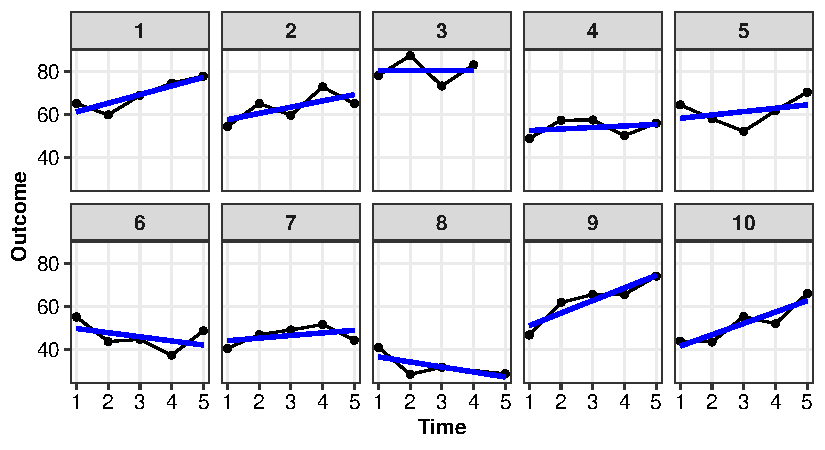
\includegraphics{lohse_ACRM_2023_module_04_files/figure-latex/figure 2-1} \end{center}

You can tinker with the values for the fixed effects, random effects,
and errors to see the effect this has on the data. For the moment
though, the goal is just to show that we can simulate longitudinal data
by reversing the process of data analysis. When analyzing data, we start
with data and try to find the best fitting fixed effects and random
effects, by minimizing the residuals (which are our best estimate of the
true errors in the population). When simulating data, we start with the
\emph{true values} of the fixed effects in the population that we
invented. We can then generate individual ``participants'' consistent
with the \emph{true} random effects (fixed effect + random deviate), and
generate individual data points based on the underlying pattern for each
participant (fixed effect + random deviate + error).

\hypertarget{simulating-two-different-populations-and-resampling-to-estimate-power}{%
\section{3. Simulating Two Different Populations and Resampling to
Estimate
Power}\label{simulating-two-different-populations-and-resampling-to-estimate-power}}

\hypertarget{setting-the-population-parameters.}{%
\subsection{3.1 Setting the population
parameters.}\label{setting-the-population-parameters.}}

Next, we will build on the same example above to simulate two different
populations. The first population (\(POP1\)) will have true intercept of
50 (sd = 10) and a true slope of 0 (sd=5).

\begin{Shaded}
\begin{Highlighting}[]
\CommentTok{\# 1.0 Set the parameters for Population 1 {-}{-}{-}{-}}
\NormalTok{N }\OtherTok{\textless{}{-}} \DecValTok{10000} \CommentTok{\# set number of individuals}

\NormalTok{beta0 }\OtherTok{\textless{}{-}} \FloatTok{50.0} \CommentTok{\# true intercept}
\NormalTok{beta1 }\OtherTok{\textless{}{-}} \FloatTok{0.0} \CommentTok{\# true slope}

\NormalTok{sigma }\OtherTok{\textless{}{-}} \DecValTok{5}  \CommentTok{\# true error SD}
\NormalTok{tau0  }\OtherTok{\textless{}{-}} \DecValTok{10}    \CommentTok{\# true intercept SD}
\NormalTok{tau1  }\OtherTok{\textless{}{-}} \DecValTok{5}  \CommentTok{\# true slope SD}
\NormalTok{tau01 }\OtherTok{\textless{}{-}} \FloatTok{0.5}  \CommentTok{\# slope{-}intercept correlation}

\CommentTok{\# number of possible observations}
\NormalTok{max\_obs }\OtherTok{\textless{}{-}} \DecValTok{5}
\NormalTok{min\_obs }\OtherTok{\textless{}{-}} \DecValTok{4}

\CommentTok{\# simulate MISSING AT RANDOM observations for each individual}
\FunctionTok{set.seed}\NormalTok{(}\DecValTok{1}\NormalTok{)}
\NormalTok{p }\OtherTok{\textless{}{-}} \FunctionTok{round}\NormalTok{(}\FunctionTok{runif}\NormalTok{(}\AttributeTok{n=}\NormalTok{N, }\AttributeTok{min=}\NormalTok{min\_obs, }\AttributeTok{max=}\NormalTok{max\_obs))}

\CommentTok{\# simulate observations per person (everyone has 1st observation)}
\NormalTok{time }\OtherTok{\textless{}{-}} \FunctionTok{unlist}\NormalTok{(}\FunctionTok{sapply}\NormalTok{(p, }\ControlFlowTok{function}\NormalTok{(x) }\FunctionTok{c}\NormalTok{(}\DecValTok{1}\NormalTok{, }\FunctionTok{sort}\NormalTok{(}\FunctionTok{sample}\NormalTok{(}\AttributeTok{x=}\DecValTok{2}\SpecialCharTok{:}\NormalTok{max\_obs, }\AttributeTok{size =}\NormalTok{ x}\DecValTok{{-}1}\NormalTok{, }\AttributeTok{replace=}\ConstantTok{FALSE}\NormalTok{)))))}

\CommentTok{\# set up data frame}
\NormalTok{POP1 }\OtherTok{\textless{}{-}} \FunctionTok{data.frame}\NormalTok{(}\AttributeTok{id=}\FunctionTok{factor}\NormalTok{(}\FunctionTok{rep}\NormalTok{(}\DecValTok{1}\SpecialCharTok{:}\NormalTok{N, }\AttributeTok{times=}\NormalTok{p)), }\AttributeTok{time=}\NormalTok{time) }\SpecialCharTok{\%\textgreater{}\%}
  \FunctionTok{mutate}\NormalTok{(}\AttributeTok{id =} \FunctionTok{factor}\NormalTok{(}\FunctionTok{paste}\NormalTok{(}\StringTok{"s1"}\NormalTok{, id, }\AttributeTok{sep=}\StringTok{"\_"}\NormalTok{)),}
         \AttributeTok{group=}\StringTok{"A"}\NormalTok{)}

\CommentTok{\# simulate (correlated) random effects for intercepts and slopes}
\NormalTok{mu  }\OtherTok{\textless{}{-}} \FunctionTok{c}\NormalTok{(}\DecValTok{0}\NormalTok{,}\DecValTok{0}\NormalTok{)}
\NormalTok{S   }\OtherTok{\textless{}{-}} \FunctionTok{matrix}\NormalTok{(}\FunctionTok{c}\NormalTok{(}\DecValTok{1}\NormalTok{, tau01, tau01, }\DecValTok{1}\NormalTok{), }\AttributeTok{nrow=}\DecValTok{2}\NormalTok{)}
\NormalTok{taus }\OtherTok{\textless{}{-}} \FunctionTok{c}\NormalTok{(tau0, tau1)}
\NormalTok{S   }\OtherTok{\textless{}{-}} \FunctionTok{diag}\NormalTok{(taus) }\SpecialCharTok{\%*\%}\NormalTok{ S }\SpecialCharTok{\%*\%} \FunctionTok{diag}\NormalTok{(taus)}
\NormalTok{U   }\OtherTok{\textless{}{-}} \FunctionTok{mvrnorm}\NormalTok{(N, }\AttributeTok{mu=}\NormalTok{mu, }\AttributeTok{Sigma=}\NormalTok{S)}

\CommentTok{\# simulate (uncorrelated) residuals}
\CommentTok{\# you can simulate correlated residuals, but that takes a bit more work}
\FunctionTok{set.seed}\NormalTok{(}\DecValTok{2}\NormalTok{)}
\NormalTok{POP1}\SpecialCharTok{$}\NormalTok{eij }\OtherTok{\textless{}{-}} \FunctionTok{rnorm}\NormalTok{(}\AttributeTok{n=}\FunctionTok{nrow}\NormalTok{(POP1), }\AttributeTok{mean=}\DecValTok{0}\NormalTok{, }\AttributeTok{sd=}\NormalTok{sigma)}

\NormalTok{POP1}\SpecialCharTok{$}\NormalTok{yij }\OtherTok{\textless{}{-}}\NormalTok{ (beta0 }\SpecialCharTok{+} \FunctionTok{rep}\NormalTok{(U[,}\DecValTok{1}\NormalTok{], }\AttributeTok{times=}\NormalTok{p)) }\SpecialCharTok{+} 
\NormalTok{  (beta1 }\SpecialCharTok{+} \FunctionTok{rep}\NormalTok{(U[,}\DecValTok{2}\NormalTok{], }\AttributeTok{times=}\NormalTok{p)) }\SpecialCharTok{*}\NormalTok{ POP1}\SpecialCharTok{$}\NormalTok{time }\SpecialCharTok{+}\NormalTok{ POP1}\SpecialCharTok{$}\NormalTok{eij}
\end{Highlighting}
\end{Shaded}

The second population (\(POP2\)) will have true intercept of 50 (sd =
10) and a true slope of 2.5 (sd=5).

\begin{Shaded}
\begin{Highlighting}[]
\CommentTok{\# 2.0 Set the parameters for Population 2 {-}{-}{-}{-}}
\NormalTok{N }\OtherTok{\textless{}{-}} \DecValTok{10000} \CommentTok{\# set number of individuals}

\NormalTok{beta0 }\OtherTok{\textless{}{-}} \FloatTok{50.0} \CommentTok{\# true intercept}
\NormalTok{beta1 }\OtherTok{\textless{}{-}} \FloatTok{2.5} \CommentTok{\# true slope}

\NormalTok{sigma }\OtherTok{\textless{}{-}} \DecValTok{5}  \CommentTok{\# true error SD}
\NormalTok{tau0  }\OtherTok{\textless{}{-}} \DecValTok{10}    \CommentTok{\# true intercept SD}
\NormalTok{tau1  }\OtherTok{\textless{}{-}} \DecValTok{5}  \CommentTok{\# true slope SD}
\NormalTok{tau01 }\OtherTok{\textless{}{-}} \FloatTok{0.5}  \CommentTok{\# slope{-}intercept correlation}

\CommentTok{\# number of possible observations}
\NormalTok{max\_obs }\OtherTok{\textless{}{-}} \DecValTok{5}
\NormalTok{min\_obs }\OtherTok{\textless{}{-}} \DecValTok{4}

\CommentTok{\# simulate MISSING AT RANDOM observations for each individual}
\FunctionTok{set.seed}\NormalTok{(}\DecValTok{1}\NormalTok{)}
\NormalTok{p }\OtherTok{\textless{}{-}} \FunctionTok{round}\NormalTok{(}\FunctionTok{runif}\NormalTok{(}\AttributeTok{n=}\NormalTok{N, }\AttributeTok{min=}\NormalTok{min\_obs, }\AttributeTok{max=}\NormalTok{max\_obs))}

\CommentTok{\# simulate observations per person (everyone has 1st observation)}
\NormalTok{time }\OtherTok{\textless{}{-}} \FunctionTok{unlist}\NormalTok{(}\FunctionTok{sapply}\NormalTok{(p, }\ControlFlowTok{function}\NormalTok{(x) }\FunctionTok{c}\NormalTok{(}\DecValTok{1}\NormalTok{, }\FunctionTok{sort}\NormalTok{(}\FunctionTok{sample}\NormalTok{(}\AttributeTok{x=}\DecValTok{2}\SpecialCharTok{:}\NormalTok{max\_obs, }\AttributeTok{size =}\NormalTok{ x}\DecValTok{{-}1}\NormalTok{, }\AttributeTok{replace=}\ConstantTok{FALSE}\NormalTok{)))))}

\CommentTok{\# set up data frame}
\NormalTok{POP2 }\OtherTok{\textless{}{-}} \FunctionTok{data.frame}\NormalTok{(}\AttributeTok{id=}\FunctionTok{factor}\NormalTok{(}\FunctionTok{rep}\NormalTok{(}\DecValTok{1}\SpecialCharTok{:}\NormalTok{N, }\AttributeTok{times=}\NormalTok{p)), }\AttributeTok{time=}\NormalTok{time)}\SpecialCharTok{\%\textgreater{}\%}
  \FunctionTok{mutate}\NormalTok{(}\AttributeTok{id =} \FunctionTok{factor}\NormalTok{(}\FunctionTok{paste}\NormalTok{(}\StringTok{"s2"}\NormalTok{, id, }\AttributeTok{sep=}\StringTok{"\_"}\NormalTok{)),}
         \AttributeTok{group=}\StringTok{"B"}\NormalTok{)}

\CommentTok{\# simulate (correlated) random effects for intercepts and slopes}
\NormalTok{mu  }\OtherTok{\textless{}{-}} \FunctionTok{c}\NormalTok{(}\DecValTok{0}\NormalTok{,}\DecValTok{0}\NormalTok{)}
\NormalTok{S   }\OtherTok{\textless{}{-}} \FunctionTok{matrix}\NormalTok{(}\FunctionTok{c}\NormalTok{(}\DecValTok{1}\NormalTok{, tau01, tau01, }\DecValTok{1}\NormalTok{), }\AttributeTok{nrow=}\DecValTok{2}\NormalTok{)}
\NormalTok{taus }\OtherTok{\textless{}{-}} \FunctionTok{c}\NormalTok{(tau0, tau1)}
\NormalTok{S   }\OtherTok{\textless{}{-}} \FunctionTok{diag}\NormalTok{(taus) }\SpecialCharTok{\%*\%}\NormalTok{ S }\SpecialCharTok{\%*\%} \FunctionTok{diag}\NormalTok{(taus)}
\NormalTok{U   }\OtherTok{\textless{}{-}} \FunctionTok{mvrnorm}\NormalTok{(N, }\AttributeTok{mu=}\NormalTok{mu, }\AttributeTok{Sigma=}\NormalTok{S)}

\CommentTok{\# simulate (uncorrelated) residuals}
\CommentTok{\# you can simulate correlated residuals, but that takes a bit more work}
\FunctionTok{set.seed}\NormalTok{(}\DecValTok{2}\NormalTok{)}
\NormalTok{POP2}\SpecialCharTok{$}\NormalTok{eij }\OtherTok{\textless{}{-}} \FunctionTok{rnorm}\NormalTok{(}\AttributeTok{n=}\FunctionTok{nrow}\NormalTok{(POP2), }\AttributeTok{mean=}\DecValTok{0}\NormalTok{, }\AttributeTok{sd=}\NormalTok{sigma)}

\NormalTok{POP2}\SpecialCharTok{$}\NormalTok{yij }\OtherTok{\textless{}{-}}\NormalTok{ (beta0 }\SpecialCharTok{+} \FunctionTok{rep}\NormalTok{(U[,}\DecValTok{1}\NormalTok{], }\AttributeTok{times=}\NormalTok{p)) }\SpecialCharTok{+} 
\NormalTok{  (beta1 }\SpecialCharTok{+} \FunctionTok{rep}\NormalTok{(U[,}\DecValTok{2}\NormalTok{], }\AttributeTok{times=}\NormalTok{p)) }\SpecialCharTok{*}\NormalTok{ POP1}\SpecialCharTok{$}\NormalTok{time }\SpecialCharTok{+}\NormalTok{ POP1}\SpecialCharTok{$}\NormalTok{eij}
\end{Highlighting}
\end{Shaded}

\hypertarget{repeatedly-sample-from-the-population-without-replacement.}{%
\subsection{3.2 Repeatedly sample from the population (without
replacement).}\label{repeatedly-sample-from-the-population-without-replacement.}}

Something something something\ldots{}

\begin{Shaded}
\begin{Highlighting}[]
\CommentTok{\# set sample sizes}
\NormalTok{sample\_sizes }\OtherTok{=} \FunctionTok{c}\NormalTok{(}\DecValTok{20}\NormalTok{, }\DecValTok{60}\NormalTok{)}

\CommentTok{\# set number of iterations at each sample size}
\NormalTok{k }\OtherTok{=} \DecValTok{1000}

\CommentTok{\# initialize null variables to populate:}
\NormalTok{sample\_size }\OtherTok{=} \ConstantTok{NULL}
\NormalTok{iteration }\OtherTok{=} \ConstantTok{NULL}
\NormalTok{random\_effects}\OtherTok{=}\ConstantTok{NULL}
\NormalTok{fixed\_effects}\OtherTok{=}\ConstantTok{NULL}
\NormalTok{anova\_results}\OtherTok{=}\ConstantTok{NULL}

\NormalTok{count}\OtherTok{=}\DecValTok{0}
\FunctionTok{set.seed}\NormalTok{(}\DecValTok{1}\NormalTok{)}
\ControlFlowTok{for}\NormalTok{ (size }\ControlFlowTok{in}\NormalTok{ sample\_sizes)\{}
  \CommentTok{\#print(size)}
  
  \ControlFlowTok{for}\NormalTok{ (i }\ControlFlowTok{in} \FunctionTok{c}\NormalTok{(}\DecValTok{1}\SpecialCharTok{:}\NormalTok{k)) \{}
\NormalTok{    count}\OtherTok{=}\NormalTok{count}\SpecialCharTok{+}\DecValTok{1}
    \CommentTok{\#print(count)}
    
    \CommentTok{\# Sample from each population}
\NormalTok{    SAMP1 }\OtherTok{\textless{}{-}}\NormalTok{ POP1[POP1}\SpecialCharTok{$}\NormalTok{id }\SpecialCharTok{\%in\%} \FunctionTok{sample}\NormalTok{(}\AttributeTok{x=}\FunctionTok{unique}\NormalTok{(POP1}\SpecialCharTok{$}\NormalTok{id), }\AttributeTok{size=}\NormalTok{size, }\AttributeTok{replace=}\ConstantTok{FALSE}\NormalTok{),]}
\NormalTok{    SAMP2 }\OtherTok{\textless{}{-}}\NormalTok{ POP2[POP2}\SpecialCharTok{$}\NormalTok{id }\SpecialCharTok{\%in\%} \FunctionTok{sample}\NormalTok{(}\AttributeTok{x=}\FunctionTok{unique}\NormalTok{(POP2}\SpecialCharTok{$}\NormalTok{id), }\AttributeTok{size=}\NormalTok{size, }\AttributeTok{replace=}\ConstantTok{FALSE}\NormalTok{),]}
    
    \CommentTok{\# Binding the two different samples together}
\NormalTok{    SAMPLE }\OtherTok{\textless{}{-}} \FunctionTok{rbind}\NormalTok{(SAMP1, SAMP2)}
    
    \CommentTok{\# Specify the model you want to fit}
\NormalTok{    mod }\OtherTok{\textless{}{-}} \FunctionTok{lmer}\NormalTok{(yij}\SpecialCharTok{\textasciitilde{}}\DecValTok{1}\SpecialCharTok{+}\NormalTok{time}\SpecialCharTok{*}\NormalTok{group}\SpecialCharTok{+}\NormalTok{(}\DecValTok{1}\SpecialCharTok{+}\NormalTok{time}\SpecialCharTok{|}\NormalTok{id), }
            \AttributeTok{data=}\NormalTok{SAMPLE, }
            \AttributeTok{REML=}\ConstantTok{TRUE}\NormalTok{)}
    
\NormalTok{    sample\_size[[count]] }\OtherTok{=}\NormalTok{ size}
\NormalTok{    iteration[[count]] }\OtherTok{=}\NormalTok{ count}
\NormalTok{    random\_effects[[count]] }\OtherTok{=} \FunctionTok{data.frame}\NormalTok{(}\FunctionTok{VarCorr}\NormalTok{(mod))}
\NormalTok{    fixed\_effects[[count]] }\OtherTok{=} \FunctionTok{data.frame}\NormalTok{(}\FunctionTok{fixef}\NormalTok{(mod))}
\NormalTok{    anova\_results[[count]] }\OtherTok{=} \FunctionTok{data.frame}\NormalTok{(}\FunctionTok{anova}\NormalTok{(mod))}
\NormalTok{  \}}
\NormalTok{\}}
\end{Highlighting}
\end{Shaded}

\begin{verbatim}
## boundary (singular) fit: see help('isSingular')
\end{verbatim}

Converting results from lists to dataframes\ldots{}

\begin{Shaded}
\begin{Highlighting}[]
\CommentTok{\# Bind all of our lists together into one big list}
\NormalTok{SIM\_RESULTS }\OtherTok{\textless{}{-}} \FunctionTok{list}\NormalTok{(}\AttributeTok{sample\_size=}\NormalTok{sample\_size,}
                    \AttributeTok{iteration=}\NormalTok{iteration,}
                    \AttributeTok{random\_effects=}\NormalTok{random\_effects,}
                    \AttributeTok{fixed\_effects=}\NormalTok{fixed\_effects,}
                    \AttributeTok{anova\_results=}\NormalTok{anova\_results)}

\CommentTok{\# Flatten out the iteration number and sample size into their own data frame}
\NormalTok{SAMP }\OtherTok{\textless{}{-}} \FunctionTok{data.frame}\NormalTok{(}\AttributeTok{iteration =} \FunctionTok{as.character}\NormalTok{(}\FunctionTok{unlist}\NormalTok{(SIM\_RESULTS}\SpecialCharTok{$}\NormalTok{iteration)),}
                   \AttributeTok{sample\_size =} \FunctionTok{unlist}\NormalTok{(SIM\_RESULTS}\SpecialCharTok{$}\NormalTok{sample\_size))}


\CommentTok{\# Tidying the random effects output}
\NormalTok{RE\_DATA }\OtherTok{\textless{}{-}} \FunctionTok{bind\_rows}\NormalTok{(SIM\_RESULTS}\SpecialCharTok{$}\NormalTok{random\_effects, }\AttributeTok{.id =} \StringTok{"iteration"}\NormalTok{) }\SpecialCharTok{\%\textgreater{}\%}
  \FunctionTok{pivot\_wider}\NormalTok{(}\AttributeTok{values\_from =}\NormalTok{ vcov}\SpecialCharTok{:}\NormalTok{sdcor, }\AttributeTok{names\_from =}\NormalTok{ grp}\SpecialCharTok{:}\NormalTok{var2, }\AttributeTok{names\_sep=}\StringTok{"\_"}\NormalTok{) }\SpecialCharTok{\%\textgreater{}\%}
  \FunctionTok{left\_join}\NormalTok{(SAMP, }\AttributeTok{by=}\StringTok{"iteration"}\NormalTok{) }\SpecialCharTok{\%\textgreater{}\%}
  \FunctionTok{relocate}\NormalTok{(iteration, sample\_size)}

\CommentTok{\# Tidying the fixed effects output}
\NormalTok{FE\_DATA }\OtherTok{\textless{}{-}} \FunctionTok{bind\_rows}\NormalTok{(SIM\_RESULTS}\SpecialCharTok{$}\NormalTok{fixed\_effects, }\AttributeTok{.id =} \StringTok{"iteration"}\NormalTok{) }\SpecialCharTok{\%\textgreater{}\%}
  \FunctionTok{rownames\_to\_column}\NormalTok{(}\AttributeTok{var=}\StringTok{"parameter"}\NormalTok{) }\SpecialCharTok{\%\textgreater{}\%}
  \FunctionTok{mutate}\NormalTok{(}\AttributeTok{parameter=}\FunctionTok{str\_split}\NormalTok{(parameter, }\StringTok{"}\SpecialCharTok{\textbackslash{}\textbackslash{}}\StringTok{.\{2,\}"}\NormalTok{, }\AttributeTok{simplify =} \ConstantTok{TRUE}\NormalTok{)[,}\DecValTok{1}\NormalTok{]) }\SpecialCharTok{\%\textgreater{}\%}
  \FunctionTok{pivot\_wider}\NormalTok{(}\AttributeTok{values\_from =}\NormalTok{ fixef.mod., }\AttributeTok{names\_from =}\NormalTok{ parameter, }\AttributeTok{names\_sep=}\StringTok{"\_"}\NormalTok{) }\SpecialCharTok{\%\textgreater{}\%}
  \FunctionTok{left\_join}\NormalTok{(SAMP, }\AttributeTok{by=}\StringTok{"iteration"}\NormalTok{) }\SpecialCharTok{\%\textgreater{}\%}
  \FunctionTok{relocate}\NormalTok{(iteration, sample\_size)}

\CommentTok{\# Tidying the ANOVA results}
\NormalTok{ANOVA\_DATA }\OtherTok{\textless{}{-}} \FunctionTok{bind\_rows}\NormalTok{(SIM\_RESULTS}\SpecialCharTok{$}\NormalTok{anova\_results, }\AttributeTok{.id =} \StringTok{"iteration"}\NormalTok{)   }\SpecialCharTok{\%\textgreater{}\%}
  \FunctionTok{rownames\_to\_column}\NormalTok{(}\AttributeTok{var=}\StringTok{"parameter"}\NormalTok{) }\SpecialCharTok{\%\textgreater{}\%}
  \FunctionTok{mutate}\NormalTok{(}\AttributeTok{parameter=}\FunctionTok{str\_split}\NormalTok{(parameter, }\StringTok{"}\SpecialCharTok{\textbackslash{}\textbackslash{}}\StringTok{.\{2,\}"}\NormalTok{, }\AttributeTok{simplify =} \ConstantTok{TRUE}\NormalTok{)[,}\DecValTok{1}\NormalTok{]) }\SpecialCharTok{\%\textgreater{}\%}
  \FunctionTok{left\_join}\NormalTok{(SAMP, }\AttributeTok{by=}\StringTok{"iteration"}\NormalTok{) }\SpecialCharTok{\%\textgreater{}\%}
  \FunctionTok{relocate}\NormalTok{(iteration, sample\_size)}


\FunctionTok{head}\NormalTok{(RE\_DATA)}
\end{Highlighting}
\end{Shaded}

\begin{verbatim}
## # A tibble: 6 x 10
##   iteration sample_size `vcov_id_(Intercept)_~` vcov_id_time_NA `vcov_id_(Inte~`
##   <chr>           <dbl>                   <dbl>           <dbl>            <dbl>
## 1 1                  20                    95.6            21.4            20.4 
## 2 2                  20                   124.             28.2            35.6 
## 3 3                  20                   117.             19.4            22.2 
## 4 4                  20                   118.             21.6            28.8 
## 5 5                  20                   157.             21.7             8.04
## 6 6                  20                    61.7            18.4            19.5 
## # ... with 5 more variables: vcov_Residual_NA_NA <dbl>,
## #   `sdcor_id_(Intercept)_NA` <dbl>, sdcor_id_time_NA <dbl>,
## #   `sdcor_id_(Intercept)_time` <dbl>, sdcor_Residual_NA_NA <dbl>
\end{verbatim}

\begin{Shaded}
\begin{Highlighting}[]
\FunctionTok{head}\NormalTok{(FE\_DATA)}
\end{Highlighting}
\end{Shaded}

\begin{verbatim}
## # A tibble: 6 x 6
##   iteration sample_size `(Intercept)`   time groupB `time:groupB`
##   <chr>           <dbl>         <dbl>  <dbl>  <dbl>         <dbl>
## 1 1                  20          50.8 -0.275 -1.12           3.39
## 2 2                  20          49.9 -1.79  -0.637          4.69
## 3 3                  20          50.2 -1.76  -0.242          3.12
## 4 4                  20          51.1 -1.32  -2.35           3.06
## 5 5                  20          50.6  0.195  1.02           3.70
## 6 6                  20          50.9  0.720 -4.51           1.58
\end{verbatim}

\begin{Shaded}
\begin{Highlighting}[]
\FunctionTok{head}\NormalTok{(ANOVA\_DATA)}
\end{Highlighting}
\end{Shaded}

\begin{verbatim}
##   iteration sample_size  parameter      Sum.Sq     Mean.Sq NumDF    DenDF
## 1         1          20       time  99.1342565  99.1342565     1 38.47797
## 2         1          20      group   2.9066550   2.9066550     1 38.37306
## 3         1          20 time:group 141.2381551 141.2381551     1 38.47797
## 4         2          20       time  10.9498976  10.9498976     1 38.29036
## 5         2          20      group   0.7198527   0.7198527     1 38.21514
## 6         2          20 time:group 194.2291131 194.2291131     1 38.29036
##      F.value     Pr..F.
## 1 3.24646582 0.07941682
## 2 0.09518764 0.75935168
## 3 4.62529159 0.03784676
## 4 0.39708094 0.53234342
## 5 0.02610433 0.87249697
## 6 7.04341557 0.01152311
\end{verbatim}

\hypertarget{estimated-statistical-power}{%
\subsection{3.3. Estimated Statistical
Power}\label{estimated-statistical-power}}

Something something something\ldots.

\begin{Shaded}
\begin{Highlighting}[]
\CommentTok{\# Plots showing the estimation of the true parameters {-}{-}{-}{-}}
\NormalTok{cbPalette }\OtherTok{\textless{}{-}} \FunctionTok{c}\NormalTok{(}\StringTok{"\#D55E00"}\NormalTok{, }\StringTok{"\#56B4E9"}\NormalTok{, }\StringTok{"\#009E73"}\NormalTok{, }\StringTok{"\#000000"}\NormalTok{, }
               \StringTok{"\#F0E442"}\NormalTok{, }\StringTok{"\#0072B2"}\NormalTok{, }\StringTok{"\#E69F00"}\NormalTok{, }\StringTok{"\#CC79A7"}\NormalTok{,}
               \StringTok{"\#999933"}\NormalTok{, }\StringTok{"\#882255"}\NormalTok{, }\StringTok{"\#661100"}\NormalTok{, }\StringTok{"\#6699CC"}\NormalTok{)}


\FunctionTok{head}\NormalTok{(ANOVA\_DATA)}
\end{Highlighting}
\end{Shaded}

\begin{verbatim}
##   iteration sample_size  parameter      Sum.Sq     Mean.Sq NumDF    DenDF
## 1         1          20       time  99.1342565  99.1342565     1 38.47797
## 2         1          20      group   2.9066550   2.9066550     1 38.37306
## 3         1          20 time:group 141.2381551 141.2381551     1 38.47797
## 4         2          20       time  10.9498976  10.9498976     1 38.29036
## 5         2          20      group   0.7198527   0.7198527     1 38.21514
## 6         2          20 time:group 194.2291131 194.2291131     1 38.29036
##      F.value     Pr..F.
## 1 3.24646582 0.07941682
## 2 0.09518764 0.75935168
## 3 4.62529159 0.03784676
## 4 0.39708094 0.53234342
## 5 0.02610433 0.87249697
## 6 7.04341557 0.01152311
\end{verbatim}

\begin{Shaded}
\begin{Highlighting}[]
\CommentTok{\# distribution of p{-}values {-}{-}{-}{-}}
\NormalTok{A}\OtherTok{\textless{}{-}}\FunctionTok{ggplot}\NormalTok{(}\AttributeTok{data=}\NormalTok{ANOVA\_DATA, }\FunctionTok{aes}\NormalTok{(}\AttributeTok{x=}\NormalTok{Pr..F.)) }\SpecialCharTok{+}
  \FunctionTok{geom\_histogram}\NormalTok{(}\FunctionTok{aes}\NormalTok{(}\AttributeTok{fill=}\NormalTok{Pr..F.}\SpecialCharTok{\textless{}}\FloatTok{0.05}\NormalTok{), }\AttributeTok{col=}\StringTok{"black"}\NormalTok{, }\AttributeTok{binwidth =} \FloatTok{0.02}\NormalTok{)}\SpecialCharTok{+}
  \FunctionTok{scale\_x\_continuous}\NormalTok{(}\AttributeTok{name =} \ConstantTok{NULL}\NormalTok{, }\AttributeTok{limits=}\FunctionTok{c}\NormalTok{(}\SpecialCharTok{{-}}\FloatTok{0.5}\NormalTok{,}\DecValTok{1}\NormalTok{)) }\SpecialCharTok{+}
  \FunctionTok{scale\_y\_continuous}\NormalTok{(}\AttributeTok{name =} \StringTok{"Frequency"}\NormalTok{) }\SpecialCharTok{+}
  \FunctionTok{ggtitle}\NormalTok{(}\AttributeTok{label=}\StringTok{"Distribution of P{-}Values"}\NormalTok{)}\SpecialCharTok{+}
  \FunctionTok{facet\_wrap}\NormalTok{(}\SpecialCharTok{\textasciitilde{}}\NormalTok{sample\_size}\SpecialCharTok{+}\NormalTok{parameter, }\AttributeTok{ncol=}\DecValTok{3}\NormalTok{, }\AttributeTok{scales =} \StringTok{"free"}\NormalTok{)}\SpecialCharTok{+}
  \FunctionTok{scale\_fill\_manual}\NormalTok{(}\AttributeTok{values=}\NormalTok{cbPalette)}\SpecialCharTok{+}
  \FunctionTok{scale\_colour\_manual}\NormalTok{(}\AttributeTok{values=}\NormalTok{cbPalette)}\SpecialCharTok{+}
  \FunctionTok{theme\_bw}\NormalTok{()}\SpecialCharTok{+}
  \FunctionTok{theme}\NormalTok{(}\AttributeTok{axis.text=}\FunctionTok{element\_text}\NormalTok{(}\AttributeTok{size=}\DecValTok{10}\NormalTok{, }\AttributeTok{color=}\StringTok{"black"}\NormalTok{),}
        \AttributeTok{legend.text=}\FunctionTok{element\_text}\NormalTok{(}\AttributeTok{size=}\DecValTok{10}\NormalTok{, }\AttributeTok{color=}\StringTok{"black"}\NormalTok{),}
        \AttributeTok{legend.title=}\FunctionTok{element\_text}\NormalTok{(}\AttributeTok{size=}\DecValTok{10}\NormalTok{, }\AttributeTok{face=}\StringTok{"bold"}\NormalTok{),}
        \AttributeTok{axis.title=}\FunctionTok{element\_text}\NormalTok{(}\AttributeTok{size=}\DecValTok{10}\NormalTok{, }\AttributeTok{face=}\StringTok{"bold"}\NormalTok{),}
        \AttributeTok{plot.title=}\FunctionTok{element\_text}\NormalTok{(}\AttributeTok{size=}\DecValTok{12}\NormalTok{, }\AttributeTok{face=}\StringTok{"bold"}\NormalTok{, }\AttributeTok{hjust=}\FloatTok{0.5}\NormalTok{),}
        \AttributeTok{panel.grid.minor =} \FunctionTok{element\_blank}\NormalTok{(),}
        \AttributeTok{strip.text =} \FunctionTok{element\_text}\NormalTok{(}\AttributeTok{size=}\DecValTok{10}\NormalTok{, }\AttributeTok{face=}\StringTok{"bold"}\NormalTok{),}
        \AttributeTok{legend.position =} \StringTok{"none"}\NormalTok{)}

\CommentTok{\# statistical power {-}{-}{-}{-}}
\NormalTok{ANOVA\_DATA }\SpecialCharTok{\%\textgreater{}\%} \FunctionTok{group\_by}\NormalTok{(sample\_size, parameter) }\SpecialCharTok{\%\textgreater{}\%}
  \FunctionTok{summarize}\NormalTok{(}\AttributeTok{sig=}\FunctionTok{sum}\NormalTok{(Pr..F.}\SpecialCharTok{\textless{}}\FloatTok{0.05}\NormalTok{)}\SpecialCharTok{/}\NormalTok{k,}
            \AttributeTok{ns=}\FunctionTok{sum}\NormalTok{(Pr..F.}\SpecialCharTok{\textgreater{}=}\FloatTok{0.05}\NormalTok{)}\SpecialCharTok{/}\NormalTok{k) }\SpecialCharTok{\%\textgreater{}\%} 
  \FunctionTok{pivot\_longer}\NormalTok{(}\AttributeTok{cols=}\NormalTok{sig}\SpecialCharTok{:}\NormalTok{ns, }\AttributeTok{names\_to =} \StringTok{"result"}\NormalTok{, }\AttributeTok{values\_to =} \StringTok{"freq"}\NormalTok{)}
\end{Highlighting}
\end{Shaded}

\begin{verbatim}
## `summarise()` has grouped output by 'sample_size'. You can override using the
## `.groups` argument.
\end{verbatim}

\begin{verbatim}
## # A tibble: 12 x 4
## # Groups:   sample_size [2]
##    sample_size parameter  result  freq
##          <dbl> <chr>      <chr>  <dbl>
##  1          20 group      sig    0.053
##  2          20 group      ns     0.947
##  3          20 time       sig    0.345
##  4          20 time       ns     0.655
##  5          20 time:group sig    0.313
##  6          20 time:group ns     0.687
##  7          60 group      sig    0.052
##  8          60 group      ns     0.948
##  9          60 time       sig    0.728
## 10          60 time       ns     0.272
## 11          60 time:group sig    0.741
## 12          60 time:group ns     0.259
\end{verbatim}

\begin{Shaded}
\begin{Highlighting}[]
\NormalTok{B}\OtherTok{\textless{}{-}}\FunctionTok{ggplot}\NormalTok{(}\AttributeTok{data=}\NormalTok{ANOVA\_DATA }\SpecialCharTok{\%\textgreater{}\%} \FunctionTok{group\_by}\NormalTok{(sample\_size, parameter) }\SpecialCharTok{\%\textgreater{}\%}
         \FunctionTok{summarize}\NormalTok{(}\AttributeTok{sig=}\FunctionTok{sum}\NormalTok{(Pr..F.}\SpecialCharTok{\textless{}}\FloatTok{0.05}\NormalTok{)}\SpecialCharTok{/}\NormalTok{k,}
                   \AttributeTok{ns=}\FunctionTok{sum}\NormalTok{(Pr..F.}\SpecialCharTok{\textgreater{}=}\FloatTok{0.05}\NormalTok{)}\SpecialCharTok{/}\NormalTok{k) }\SpecialCharTok{\%\textgreater{}\%} 
         \FunctionTok{pivot\_longer}\NormalTok{(}\AttributeTok{cols=}\NormalTok{sig}\SpecialCharTok{:}\NormalTok{ns, }\AttributeTok{names\_to =} \StringTok{"result"}\NormalTok{, }\AttributeTok{values\_to =} \StringTok{"freq"}\NormalTok{),}
       \FunctionTok{aes}\NormalTok{(}\AttributeTok{x=}\NormalTok{result, }\AttributeTok{y=}\NormalTok{freq)) }\SpecialCharTok{+}
  \FunctionTok{geom\_bar}\NormalTok{(}\FunctionTok{aes}\NormalTok{(}\AttributeTok{fill=}\NormalTok{result), }\AttributeTok{col=}\StringTok{"black"}\NormalTok{, }\AttributeTok{stat=}\StringTok{"identity"}\NormalTok{)}\SpecialCharTok{+}
  \FunctionTok{geom\_hline}\NormalTok{(}\AttributeTok{yintercept=}\FloatTok{0.8}\NormalTok{, }\AttributeTok{lty=}\DecValTok{2}\NormalTok{, }\AttributeTok{lwd=}\DecValTok{1}\NormalTok{)}\SpecialCharTok{+}
  \FunctionTok{ggtitle}\NormalTok{(}\AttributeTok{label=}\StringTok{"Statistical Power"}\NormalTok{)}\SpecialCharTok{+}
  \FunctionTok{scale\_x\_discrete}\NormalTok{(}\AttributeTok{name =} \ConstantTok{NULL}\NormalTok{) }\SpecialCharTok{+}
  \FunctionTok{scale\_y\_continuous}\NormalTok{(}\AttributeTok{name =} \StringTok{"Proportion of Results"}\NormalTok{, }\AttributeTok{limits=}\FunctionTok{c}\NormalTok{(}\DecValTok{0}\NormalTok{,}\DecValTok{1}\NormalTok{)) }\SpecialCharTok{+}
  \FunctionTok{facet\_wrap}\NormalTok{(}\SpecialCharTok{\textasciitilde{}}\NormalTok{sample\_size}\SpecialCharTok{+}\NormalTok{parameter, }\AttributeTok{ncol=}\DecValTok{3}\NormalTok{)}\SpecialCharTok{+}
  \FunctionTok{scale\_fill\_manual}\NormalTok{(}\AttributeTok{values=}\NormalTok{cbPalette)}\SpecialCharTok{+}
  \FunctionTok{scale\_colour\_manual}\NormalTok{(}\AttributeTok{values=}\NormalTok{cbPalette)}\SpecialCharTok{+}
  \FunctionTok{theme\_bw}\NormalTok{()}\SpecialCharTok{+}
  \FunctionTok{theme}\NormalTok{(}\AttributeTok{axis.text=}\FunctionTok{element\_text}\NormalTok{(}\AttributeTok{size=}\DecValTok{10}\NormalTok{, }\AttributeTok{color=}\StringTok{"black"}\NormalTok{),}
        \AttributeTok{legend.text=}\FunctionTok{element\_text}\NormalTok{(}\AttributeTok{size=}\DecValTok{10}\NormalTok{, }\AttributeTok{color=}\StringTok{"black"}\NormalTok{),}
        \AttributeTok{legend.title=}\FunctionTok{element\_text}\NormalTok{(}\AttributeTok{size=}\DecValTok{10}\NormalTok{, }\AttributeTok{face=}\StringTok{"bold"}\NormalTok{),}
        \AttributeTok{axis.title=}\FunctionTok{element\_text}\NormalTok{(}\AttributeTok{size=}\DecValTok{10}\NormalTok{, }\AttributeTok{face=}\StringTok{"bold"}\NormalTok{),}
        \AttributeTok{plot.title=}\FunctionTok{element\_text}\NormalTok{(}\AttributeTok{size=}\DecValTok{12}\NormalTok{, }\AttributeTok{face=}\StringTok{"bold"}\NormalTok{, }\AttributeTok{hjust=}\FloatTok{0.5}\NormalTok{),}
        \AttributeTok{panel.grid.minor =} \FunctionTok{element\_blank}\NormalTok{(),}
        \AttributeTok{strip.text =} \FunctionTok{element\_text}\NormalTok{(}\AttributeTok{size=}\DecValTok{10}\NormalTok{, }\AttributeTok{face=}\StringTok{"bold"}\NormalTok{),}
        \AttributeTok{legend.position =} \StringTok{"none"}\NormalTok{)}
\end{Highlighting}
\end{Shaded}

\begin{verbatim}
## `summarise()` has grouped output by 'sample_size'. You can override using the
## `.groups` argument.
\end{verbatim}

\begin{Shaded}
\begin{Highlighting}[]
\NormalTok{(A)}\SpecialCharTok{/}\NormalTok{(B)}
\end{Highlighting}
\end{Shaded}

\begin{center}\includegraphics{lohse_ACRM_2023_module_04_files/figure-latex/figure 3-1} \end{center}

\hypertarget{sampling-distribution-of-fixed-effect-estimates}{%
\subsection{3.4. Sampling Distribution of Fixed-Effect
Estimates}\label{sampling-distribution-of-fixed-effect-estimates}}

Something something something\ldots.

\begin{Shaded}
\begin{Highlighting}[]
\CommentTok{\# Plots showing the estimation of the true parameters {-}{-}{-}{-}}
\NormalTok{cbPalette }\OtherTok{\textless{}{-}} \FunctionTok{c}\NormalTok{(}\StringTok{"\#D55E00"}\NormalTok{, }\StringTok{"\#56B4E9"}\NormalTok{, }\StringTok{"\#009E73"}\NormalTok{, }\StringTok{"\#000000"}\NormalTok{, }
               \StringTok{"\#F0E442"}\NormalTok{, }\StringTok{"\#0072B2"}\NormalTok{, }\StringTok{"\#E69F00"}\NormalTok{, }\StringTok{"\#CC79A7"}\NormalTok{,}
               \StringTok{"\#999933"}\NormalTok{, }\StringTok{"\#882255"}\NormalTok{, }\StringTok{"\#661100"}\NormalTok{, }\StringTok{"\#6699CC"}\NormalTok{)}


\CommentTok{\# Group Effect at baseline {-}{-}{-}{-}}
\NormalTok{FE1 }\OtherTok{\textless{}{-}} \FunctionTok{ggplot}\NormalTok{(}\AttributeTok{data=}\NormalTok{FE\_DATA, }\FunctionTok{aes}\NormalTok{(}\AttributeTok{x=}\NormalTok{groupB)) }\SpecialCharTok{+}
  \FunctionTok{geom\_histogram}\NormalTok{(}\FunctionTok{aes}\NormalTok{(}\AttributeTok{fill=}\FunctionTok{factor}\NormalTok{(sample\_size)), }\AttributeTok{col=}\StringTok{"black"}\NormalTok{, }\AttributeTok{bins=}\DecValTok{30}\NormalTok{,}
                 \AttributeTok{position=}\StringTok{"identity"}\NormalTok{, }\AttributeTok{alpha=}\FloatTok{0.5}\NormalTok{)}\SpecialCharTok{+}
  \CommentTok{\#geom\_vline(xintercept=beta0, lty=2, lwd=1, col="black")+}
  \FunctionTok{scale\_x\_continuous}\NormalTok{(}\AttributeTok{name =} \ConstantTok{NULL}\NormalTok{) }\SpecialCharTok{+}
  \FunctionTok{scale\_y\_continuous}\NormalTok{(}\AttributeTok{name =} \StringTok{"Frequency"}\NormalTok{) }\SpecialCharTok{+}
  \FunctionTok{ggtitle}\NormalTok{(}\AttributeTok{label=}\StringTok{"Simple Effect of Group (intercept)"}\NormalTok{)}\SpecialCharTok{+}
  \FunctionTok{scale\_fill\_manual}\NormalTok{(}\AttributeTok{values=}\NormalTok{cbPalette)}\SpecialCharTok{+}
  \FunctionTok{scale\_colour\_manual}\NormalTok{(}\AttributeTok{values=}\NormalTok{cbPalette)}\SpecialCharTok{+}
  \FunctionTok{labs}\NormalTok{(}\AttributeTok{fill=}\StringTok{"Sample Size"}\NormalTok{)}\SpecialCharTok{+}
  \CommentTok{\#facet\_wrap(\textasciitilde{}sample\_size, ncol=1)+}
  \FunctionTok{theme\_bw}\NormalTok{()}\SpecialCharTok{+}
  \FunctionTok{theme}\NormalTok{(}\AttributeTok{axis.text=}\FunctionTok{element\_text}\NormalTok{(}\AttributeTok{size=}\DecValTok{10}\NormalTok{, }\AttributeTok{color=}\StringTok{"black"}\NormalTok{),}
        \AttributeTok{legend.text=}\FunctionTok{element\_text}\NormalTok{(}\AttributeTok{size=}\DecValTok{10}\NormalTok{, }\AttributeTok{color=}\StringTok{"black"}\NormalTok{),}
        \AttributeTok{legend.title=}\FunctionTok{element\_text}\NormalTok{(}\AttributeTok{size=}\DecValTok{10}\NormalTok{, }\AttributeTok{face=}\StringTok{"bold"}\NormalTok{),}
        \AttributeTok{axis.title=}\FunctionTok{element\_text}\NormalTok{(}\AttributeTok{size=}\DecValTok{10}\NormalTok{, }\AttributeTok{face=}\StringTok{"bold"}\NormalTok{),}
        \AttributeTok{plot.title=}\FunctionTok{element\_text}\NormalTok{(}\AttributeTok{size=}\DecValTok{11}\NormalTok{, }\AttributeTok{face=}\StringTok{"bold"}\NormalTok{, }\AttributeTok{hjust=}\FloatTok{0.5}\NormalTok{),}
        \AttributeTok{panel.grid.minor =} \FunctionTok{element\_blank}\NormalTok{(),}
        \AttributeTok{strip.text =} \FunctionTok{element\_text}\NormalTok{(}\AttributeTok{size=}\DecValTok{10}\NormalTok{, }\AttributeTok{face=}\StringTok{"bold"}\NormalTok{),}
        \AttributeTok{legend.position =} \StringTok{"bottom"}\NormalTok{)}

\CommentTok{\# Effect of Time in Reference Groups {-}{-}{-}{-}}
\NormalTok{FE2 }\OtherTok{\textless{}{-}} \FunctionTok{ggplot}\NormalTok{(}\AttributeTok{data=}\NormalTok{FE\_DATA, }\FunctionTok{aes}\NormalTok{(}\AttributeTok{x=}\NormalTok{time)) }\SpecialCharTok{+}
  \FunctionTok{geom\_histogram}\NormalTok{(}\FunctionTok{aes}\NormalTok{(}\AttributeTok{fill=}\FunctionTok{factor}\NormalTok{(sample\_size)), }\AttributeTok{col=}\StringTok{"black"}\NormalTok{, }\AttributeTok{bins=}\DecValTok{30}\NormalTok{,}
                 \AttributeTok{position=}\StringTok{"identity"}\NormalTok{, }\AttributeTok{alpha=}\FloatTok{0.5}\NormalTok{)}\SpecialCharTok{+}
  \CommentTok{\#geom\_vline(xintercept=beta0, lty=2, lwd=1, col="black")+}
  \FunctionTok{scale\_x\_continuous}\NormalTok{(}\AttributeTok{name =} \ConstantTok{NULL}\NormalTok{) }\SpecialCharTok{+}
  \FunctionTok{scale\_y\_continuous}\NormalTok{(}\AttributeTok{name =} \StringTok{"Frequency"}\NormalTok{) }\SpecialCharTok{+}
  \FunctionTok{ggtitle}\NormalTok{(}\AttributeTok{label=}\StringTok{"Simple Effect of Time (reference)"}\NormalTok{)}\SpecialCharTok{+}
  \FunctionTok{scale\_fill\_manual}\NormalTok{(}\AttributeTok{values=}\NormalTok{cbPalette)}\SpecialCharTok{+}
  \FunctionTok{scale\_colour\_manual}\NormalTok{(}\AttributeTok{values=}\NormalTok{cbPalette)}\SpecialCharTok{+}
  \FunctionTok{labs}\NormalTok{(}\AttributeTok{fill=}\StringTok{"Sample Size"}\NormalTok{)}\SpecialCharTok{+}
  \CommentTok{\#facet\_wrap(\textasciitilde{}sample\_size, ncol=1)+}
  \FunctionTok{theme\_bw}\NormalTok{()}\SpecialCharTok{+}
  \FunctionTok{theme}\NormalTok{(}\AttributeTok{axis.text=}\FunctionTok{element\_text}\NormalTok{(}\AttributeTok{size=}\DecValTok{10}\NormalTok{, }\AttributeTok{color=}\StringTok{"black"}\NormalTok{),}
        \AttributeTok{legend.text=}\FunctionTok{element\_text}\NormalTok{(}\AttributeTok{size=}\DecValTok{10}\NormalTok{, }\AttributeTok{color=}\StringTok{"black"}\NormalTok{),}
        \AttributeTok{legend.title=}\FunctionTok{element\_text}\NormalTok{(}\AttributeTok{size=}\DecValTok{10}\NormalTok{, }\AttributeTok{face=}\StringTok{"bold"}\NormalTok{),}
        \AttributeTok{axis.title=}\FunctionTok{element\_text}\NormalTok{(}\AttributeTok{size=}\DecValTok{10}\NormalTok{, }\AttributeTok{face=}\StringTok{"bold"}\NormalTok{),}
        \AttributeTok{plot.title=}\FunctionTok{element\_text}\NormalTok{(}\AttributeTok{size=}\DecValTok{11}\NormalTok{, }\AttributeTok{face=}\StringTok{"bold"}\NormalTok{, }\AttributeTok{hjust=}\FloatTok{0.5}\NormalTok{),}
        \AttributeTok{panel.grid.minor =} \FunctionTok{element\_blank}\NormalTok{(),}
        \AttributeTok{strip.text =} \FunctionTok{element\_text}\NormalTok{(}\AttributeTok{size=}\DecValTok{10}\NormalTok{, }\AttributeTok{face=}\StringTok{"bold"}\NormalTok{),}
        \AttributeTok{legend.position =} \StringTok{"bottom"}\NormalTok{)}

\CommentTok{\# Difference between slopes {-}{-}{-}{-}}
\NormalTok{FE3 }\OtherTok{\textless{}{-}} \FunctionTok{ggplot}\NormalTok{(}\AttributeTok{data=}\NormalTok{FE\_DATA, }\FunctionTok{aes}\NormalTok{(}\AttributeTok{x=}\StringTok{\textasciigrave{}}\AttributeTok{time:groupB}\StringTok{\textasciigrave{}}\NormalTok{)) }\SpecialCharTok{+}
  \FunctionTok{geom\_histogram}\NormalTok{(}\FunctionTok{aes}\NormalTok{(}\AttributeTok{fill=}\FunctionTok{factor}\NormalTok{(sample\_size)), }\AttributeTok{col=}\StringTok{"black"}\NormalTok{, }\AttributeTok{bins=}\DecValTok{30}\NormalTok{,}
                 \AttributeTok{position=}\StringTok{"identity"}\NormalTok{, }\AttributeTok{alpha=}\FloatTok{0.5}\NormalTok{)}\SpecialCharTok{+}
  \CommentTok{\#geom\_vline(xintercept=beta1, lty=2, lwd=1, col="black")+}
  \FunctionTok{scale\_x\_continuous}\NormalTok{(}\AttributeTok{name =} \ConstantTok{NULL}\NormalTok{) }\SpecialCharTok{+}
  \FunctionTok{scale\_y\_continuous}\NormalTok{(}\AttributeTok{name =} \StringTok{"Frequency"}\NormalTok{) }\SpecialCharTok{+}
  \FunctionTok{ggtitle}\NormalTok{(}\AttributeTok{label=}\StringTok{"Group x Time Interaction"}\NormalTok{)}\SpecialCharTok{+}
  \FunctionTok{scale\_fill\_manual}\NormalTok{(}\AttributeTok{values=}\NormalTok{cbPalette)}\SpecialCharTok{+}
  \FunctionTok{scale\_colour\_manual}\NormalTok{(}\AttributeTok{values=}\NormalTok{cbPalette)}\SpecialCharTok{+}
  \FunctionTok{labs}\NormalTok{(}\AttributeTok{fill=}\StringTok{"Sample Size"}\NormalTok{)}\SpecialCharTok{+}
  \CommentTok{\#facet\_wrap(\textasciitilde{}sample\_size, ncol=1)+}
  \FunctionTok{theme\_bw}\NormalTok{()}\SpecialCharTok{+}
  \FunctionTok{theme}\NormalTok{(}\AttributeTok{axis.text=}\FunctionTok{element\_text}\NormalTok{(}\AttributeTok{size=}\DecValTok{10}\NormalTok{, }\AttributeTok{color=}\StringTok{"black"}\NormalTok{),}
        \AttributeTok{legend.text=}\FunctionTok{element\_text}\NormalTok{(}\AttributeTok{size=}\DecValTok{10}\NormalTok{, }\AttributeTok{color=}\StringTok{"black"}\NormalTok{),}
        \AttributeTok{legend.title=}\FunctionTok{element\_text}\NormalTok{(}\AttributeTok{size=}\DecValTok{10}\NormalTok{, }\AttributeTok{face=}\StringTok{"bold"}\NormalTok{),}
        \AttributeTok{axis.title=}\FunctionTok{element\_text}\NormalTok{(}\AttributeTok{size=}\DecValTok{10}\NormalTok{, }\AttributeTok{face=}\StringTok{"bold"}\NormalTok{),}
        \AttributeTok{plot.title=}\FunctionTok{element\_text}\NormalTok{(}\AttributeTok{size=}\DecValTok{11}\NormalTok{, }\AttributeTok{face=}\StringTok{"bold"}\NormalTok{, }\AttributeTok{hjust=}\FloatTok{0.5}\NormalTok{),}
        \AttributeTok{panel.grid.minor =} \FunctionTok{element\_blank}\NormalTok{(),}
        \AttributeTok{strip.text =} \FunctionTok{element\_text}\NormalTok{(}\AttributeTok{size=}\DecValTok{10}\NormalTok{, }\AttributeTok{face=}\StringTok{"bold"}\NormalTok{),}
        \AttributeTok{legend.position =} \StringTok{"bottom"}\NormalTok{)}

\NormalTok{FE1}\SpecialCharTok{|}\NormalTok{FE2}\SpecialCharTok{|}\NormalTok{FE3}
\end{Highlighting}
\end{Shaded}

\begin{center}\includegraphics{lohse_ACRM_2023_module_04_files/figure-latex/figure 4-1} \end{center}

\hypertarget{sampling-distribution-of-random-effect-estimates}{%
\subsection{3.5. Sampling Distribution of Random-Effect
Estimates}\label{sampling-distribution-of-random-effect-estimates}}

Something something something\ldots.

\begin{Shaded}
\begin{Highlighting}[]
\CommentTok{\# Plots showing the estimation of the true parameters {-}{-}{-}{-}}
\NormalTok{cbPalette }\OtherTok{\textless{}{-}} \FunctionTok{c}\NormalTok{(}\StringTok{"\#D55E00"}\NormalTok{, }\StringTok{"\#56B4E9"}\NormalTok{, }\StringTok{"\#009E73"}\NormalTok{, }\StringTok{"\#000000"}\NormalTok{, }
               \StringTok{"\#F0E442"}\NormalTok{, }\StringTok{"\#0072B2"}\NormalTok{, }\StringTok{"\#E69F00"}\NormalTok{, }\StringTok{"\#CC79A7"}\NormalTok{,}
               \StringTok{"\#999933"}\NormalTok{, }\StringTok{"\#882255"}\NormalTok{, }\StringTok{"\#661100"}\NormalTok{, }\StringTok{"\#6699CC"}\NormalTok{)}


\CommentTok{\# tau0  true standard deviation of the random intercept {-}{-}{-}{-}}
\NormalTok{RE1}\OtherTok{\textless{}{-}}\FunctionTok{ggplot}\NormalTok{(}\AttributeTok{data=}\NormalTok{RE\_DATA, }\FunctionTok{aes}\NormalTok{(}\AttributeTok{x=}\StringTok{\textasciigrave{}}\AttributeTok{sdcor\_id\_(Intercept)\_NA}\StringTok{\textasciigrave{}}\NormalTok{)) }\SpecialCharTok{+}
  \FunctionTok{geom\_histogram}\NormalTok{(}\FunctionTok{aes}\NormalTok{(}\AttributeTok{fill=}\FunctionTok{factor}\NormalTok{(sample\_size)), }\AttributeTok{col=}\StringTok{"black"}\NormalTok{, }\AttributeTok{bins=}\DecValTok{30}\NormalTok{,}
                 \AttributeTok{position=}\StringTok{"identity"}\NormalTok{, }\AttributeTok{alpha=}\FloatTok{0.5}\NormalTok{)}\SpecialCharTok{+}
  \FunctionTok{geom\_vline}\NormalTok{(}\AttributeTok{xintercept=}\NormalTok{tau0, }\AttributeTok{lty=}\DecValTok{2}\NormalTok{, }\AttributeTok{lwd=}\DecValTok{1}\NormalTok{, }\AttributeTok{col=}\StringTok{"black"}\NormalTok{)}\SpecialCharTok{+}
  \FunctionTok{scale\_x\_continuous}\NormalTok{(}\AttributeTok{name =} \ConstantTok{NULL}\NormalTok{) }\SpecialCharTok{+}
  \FunctionTok{scale\_y\_continuous}\NormalTok{(}\AttributeTok{name =} \StringTok{"Frequency"}\NormalTok{) }\SpecialCharTok{+}
  \FunctionTok{ggtitle}\NormalTok{(}\AttributeTok{label=}\StringTok{"Random Intercept SD"}\NormalTok{)}\SpecialCharTok{+}
  \FunctionTok{scale\_fill\_manual}\NormalTok{(}\AttributeTok{values=}\NormalTok{cbPalette)}\SpecialCharTok{+}
  \FunctionTok{scale\_colour\_manual}\NormalTok{(}\AttributeTok{values=}\NormalTok{cbPalette)}\SpecialCharTok{+}
  \FunctionTok{labs}\NormalTok{(}\AttributeTok{fill=}\StringTok{"Sample Size"}\NormalTok{)}\SpecialCharTok{+}
  \CommentTok{\#facet\_wrap(\textasciitilde{}sample\_size, ncol=1)+}
  \FunctionTok{theme\_bw}\NormalTok{()}\SpecialCharTok{+}
  \FunctionTok{theme}\NormalTok{(}\AttributeTok{axis.text=}\FunctionTok{element\_text}\NormalTok{(}\AttributeTok{size=}\DecValTok{10}\NormalTok{, }\AttributeTok{color=}\StringTok{"black"}\NormalTok{),}
        \AttributeTok{legend.text=}\FunctionTok{element\_text}\NormalTok{(}\AttributeTok{size=}\DecValTok{10}\NormalTok{, }\AttributeTok{color=}\StringTok{"black"}\NormalTok{),}
        \AttributeTok{legend.title=}\FunctionTok{element\_text}\NormalTok{(}\AttributeTok{size=}\DecValTok{10}\NormalTok{, }\AttributeTok{face=}\StringTok{"bold"}\NormalTok{),}
        \AttributeTok{axis.title=}\FunctionTok{element\_text}\NormalTok{(}\AttributeTok{size=}\DecValTok{10}\NormalTok{, }\AttributeTok{face=}\StringTok{"bold"}\NormalTok{),}
        \AttributeTok{plot.title=}\FunctionTok{element\_text}\NormalTok{(}\AttributeTok{size=}\DecValTok{11}\NormalTok{, }\AttributeTok{face=}\StringTok{"bold"}\NormalTok{, }\AttributeTok{hjust=}\FloatTok{0.5}\NormalTok{),}
        \AttributeTok{panel.grid.minor =} \FunctionTok{element\_blank}\NormalTok{(),}
        \AttributeTok{strip.text =} \FunctionTok{element\_text}\NormalTok{(}\AttributeTok{size=}\DecValTok{10}\NormalTok{, }\AttributeTok{face=}\StringTok{"bold"}\NormalTok{),}
        \AttributeTok{legend.position =} \StringTok{"none"}\NormalTok{)}

\CommentTok{\# tau1 true standard deviation of the random slope {-}{-}{-}{-}}
\NormalTok{RE2 }\OtherTok{\textless{}{-}} \FunctionTok{ggplot}\NormalTok{(}\AttributeTok{data=}\NormalTok{RE\_DATA, }\FunctionTok{aes}\NormalTok{(}\AttributeTok{x=}\StringTok{\textasciigrave{}}\AttributeTok{sdcor\_id\_time\_NA}\StringTok{\textasciigrave{}}\NormalTok{)) }\SpecialCharTok{+}
  \FunctionTok{geom\_histogram}\NormalTok{(}\FunctionTok{aes}\NormalTok{(}\AttributeTok{fill=}\FunctionTok{factor}\NormalTok{(sample\_size)), }\AttributeTok{col=}\StringTok{"black"}\NormalTok{, }\AttributeTok{bins=}\DecValTok{30}\NormalTok{,}
                 \AttributeTok{position=}\StringTok{"identity"}\NormalTok{, }\AttributeTok{alpha=}\FloatTok{0.5}\NormalTok{)}\SpecialCharTok{+}
  \FunctionTok{geom\_vline}\NormalTok{(}\AttributeTok{xintercept=}\NormalTok{tau1, }\AttributeTok{lty=}\DecValTok{2}\NormalTok{, }\AttributeTok{lwd=}\DecValTok{1}\NormalTok{, }\AttributeTok{col=}\StringTok{"black"}\NormalTok{)}\SpecialCharTok{+}
  \FunctionTok{scale\_x\_continuous}\NormalTok{(}\AttributeTok{name =} \ConstantTok{NULL}\NormalTok{) }\SpecialCharTok{+}
  \FunctionTok{scale\_y\_continuous}\NormalTok{(}\AttributeTok{name =} \StringTok{"Frequency"}\NormalTok{) }\SpecialCharTok{+}
  \FunctionTok{ggtitle}\NormalTok{(}\AttributeTok{label=}\StringTok{"Random Slope SD"}\NormalTok{)}\SpecialCharTok{+}
  \FunctionTok{scale\_fill\_manual}\NormalTok{(}\AttributeTok{values=}\NormalTok{cbPalette)}\SpecialCharTok{+}
  \FunctionTok{scale\_colour\_manual}\NormalTok{(}\AttributeTok{values=}\NormalTok{cbPalette)}\SpecialCharTok{+}
  \FunctionTok{labs}\NormalTok{(}\AttributeTok{fill=}\StringTok{"Sample Size"}\NormalTok{)}\SpecialCharTok{+}
  \CommentTok{\#facet\_wrap(\textasciitilde{}sample\_size, ncol=1)+}
  \FunctionTok{theme\_bw}\NormalTok{()}\SpecialCharTok{+}
  \FunctionTok{theme}\NormalTok{(}\AttributeTok{axis.text=}\FunctionTok{element\_text}\NormalTok{(}\AttributeTok{size=}\DecValTok{10}\NormalTok{, }\AttributeTok{color=}\StringTok{"black"}\NormalTok{),}
        \AttributeTok{legend.text=}\FunctionTok{element\_text}\NormalTok{(}\AttributeTok{size=}\DecValTok{10}\NormalTok{, }\AttributeTok{color=}\StringTok{"black"}\NormalTok{),}
        \AttributeTok{legend.title=}\FunctionTok{element\_text}\NormalTok{(}\AttributeTok{size=}\DecValTok{10}\NormalTok{, }\AttributeTok{face=}\StringTok{"bold"}\NormalTok{),}
        \AttributeTok{axis.title=}\FunctionTok{element\_text}\NormalTok{(}\AttributeTok{size=}\DecValTok{10}\NormalTok{, }\AttributeTok{face=}\StringTok{"bold"}\NormalTok{),}
        \AttributeTok{plot.title=}\FunctionTok{element\_text}\NormalTok{(}\AttributeTok{size=}\DecValTok{11}\NormalTok{, }\AttributeTok{face=}\StringTok{"bold"}\NormalTok{, }\AttributeTok{hjust=}\FloatTok{0.5}\NormalTok{),}
        \AttributeTok{panel.grid.minor =} \FunctionTok{element\_blank}\NormalTok{(),}
        \AttributeTok{strip.text =} \FunctionTok{element\_text}\NormalTok{(}\AttributeTok{size=}\DecValTok{10}\NormalTok{, }\AttributeTok{face=}\StringTok{"bold"}\NormalTok{),}
        \AttributeTok{legend.position =} \StringTok{"none"}\NormalTok{)}

\CommentTok{\# tau01 true correlation between random{-}slopes/intercepts {-}{-}{-}{-}}
\NormalTok{RE3}\OtherTok{\textless{}{-}}\FunctionTok{ggplot}\NormalTok{(}\AttributeTok{data=}\NormalTok{RE\_DATA, }\FunctionTok{aes}\NormalTok{(}\AttributeTok{x=}\StringTok{\textasciigrave{}}\AttributeTok{sdcor\_id\_(Intercept)\_time}\StringTok{\textasciigrave{}}\NormalTok{)) }\SpecialCharTok{+}
  \FunctionTok{geom\_histogram}\NormalTok{(}\FunctionTok{aes}\NormalTok{(}\AttributeTok{fill=}\FunctionTok{factor}\NormalTok{(sample\_size)), }\AttributeTok{col=}\StringTok{"black"}\NormalTok{, }\AttributeTok{bins=}\DecValTok{30}\NormalTok{,}
                 \AttributeTok{position=}\StringTok{"identity"}\NormalTok{, }\AttributeTok{alpha=}\FloatTok{0.5}\NormalTok{)}\SpecialCharTok{+}
  \FunctionTok{geom\_vline}\NormalTok{(}\AttributeTok{xintercept=}\NormalTok{tau01, }\AttributeTok{lty=}\DecValTok{2}\NormalTok{, }\AttributeTok{lwd=}\DecValTok{1}\NormalTok{, }\AttributeTok{col=}\StringTok{"black"}\NormalTok{)}\SpecialCharTok{+}
  \FunctionTok{scale\_x\_continuous}\NormalTok{(}\AttributeTok{name =} \ConstantTok{NULL}\NormalTok{) }\SpecialCharTok{+}
  \FunctionTok{scale\_y\_continuous}\NormalTok{(}\AttributeTok{name =} \StringTok{"Frequency"}\NormalTok{) }\SpecialCharTok{+}
  \FunctionTok{ggtitle}\NormalTok{(}\AttributeTok{label=}\StringTok{"Correlation (Slopes\textasciitilde{}Intercepts)"}\NormalTok{)}\SpecialCharTok{+}
  \FunctionTok{scale\_fill\_manual}\NormalTok{(}\AttributeTok{values=}\NormalTok{cbPalette)}\SpecialCharTok{+}
  \FunctionTok{scale\_colour\_manual}\NormalTok{(}\AttributeTok{values=}\NormalTok{cbPalette)}\SpecialCharTok{+}
  \FunctionTok{labs}\NormalTok{(}\AttributeTok{fill=}\StringTok{"Sample Size"}\NormalTok{)}\SpecialCharTok{+}
  \CommentTok{\#facet\_wrap(\textasciitilde{}sample\_size, ncol=1)+}
  \FunctionTok{theme\_bw}\NormalTok{()}\SpecialCharTok{+}
  \FunctionTok{theme}\NormalTok{(}\AttributeTok{axis.text=}\FunctionTok{element\_text}\NormalTok{(}\AttributeTok{size=}\DecValTok{10}\NormalTok{, }\AttributeTok{color=}\StringTok{"black"}\NormalTok{),}
        \AttributeTok{legend.text=}\FunctionTok{element\_text}\NormalTok{(}\AttributeTok{size=}\DecValTok{10}\NormalTok{, }\AttributeTok{color=}\StringTok{"black"}\NormalTok{),}
        \AttributeTok{legend.title=}\FunctionTok{element\_text}\NormalTok{(}\AttributeTok{size=}\DecValTok{10}\NormalTok{, }\AttributeTok{face=}\StringTok{"bold"}\NormalTok{),}
        \AttributeTok{axis.title=}\FunctionTok{element\_text}\NormalTok{(}\AttributeTok{size=}\DecValTok{10}\NormalTok{, }\AttributeTok{face=}\StringTok{"bold"}\NormalTok{),}
        \AttributeTok{plot.title=}\FunctionTok{element\_text}\NormalTok{(}\AttributeTok{size=}\DecValTok{11}\NormalTok{, }\AttributeTok{face=}\StringTok{"bold"}\NormalTok{, }\AttributeTok{hjust=}\FloatTok{0.5}\NormalTok{),}
        \AttributeTok{panel.grid.minor =} \FunctionTok{element\_blank}\NormalTok{(),}
        \AttributeTok{strip.text =} \FunctionTok{element\_text}\NormalTok{(}\AttributeTok{size=}\DecValTok{10}\NormalTok{, }\AttributeTok{face=}\StringTok{"bold"}\NormalTok{),}
        \AttributeTok{legend.position =} \StringTok{"bottom"}\NormalTok{)}


\CommentTok{\# sigma true standard deviation of the residuals {-}{-}{-}{-}}
\NormalTok{RE4}\OtherTok{\textless{}{-}}\FunctionTok{ggplot}\NormalTok{(}\AttributeTok{data=}\NormalTok{RE\_DATA, }\FunctionTok{aes}\NormalTok{(}\AttributeTok{x=}\NormalTok{sdcor\_Residual\_NA\_NA)) }\SpecialCharTok{+}
  \FunctionTok{geom\_histogram}\NormalTok{(}\FunctionTok{aes}\NormalTok{(}\AttributeTok{fill=}\FunctionTok{factor}\NormalTok{(sample\_size)), }\AttributeTok{col=}\StringTok{"black"}\NormalTok{, }\AttributeTok{bins=}\DecValTok{30}\NormalTok{,}
                 \AttributeTok{position=}\StringTok{"identity"}\NormalTok{, }\AttributeTok{alpha=}\FloatTok{0.5}\NormalTok{)}\SpecialCharTok{+}
  \FunctionTok{geom\_vline}\NormalTok{(}\AttributeTok{xintercept=}\NormalTok{sigma, }\AttributeTok{lty=}\DecValTok{2}\NormalTok{, }\AttributeTok{lwd=}\DecValTok{1}\NormalTok{, }\AttributeTok{col=}\StringTok{"black"}\NormalTok{)}\SpecialCharTok{+}
  \FunctionTok{scale\_x\_continuous}\NormalTok{(}\AttributeTok{name =} \ConstantTok{NULL}\NormalTok{) }\SpecialCharTok{+}
  \FunctionTok{scale\_y\_continuous}\NormalTok{(}\AttributeTok{name =} \StringTok{"Frequency"}\NormalTok{) }\SpecialCharTok{+}
  \FunctionTok{ggtitle}\NormalTok{(}\AttributeTok{label=}\StringTok{"Residual SD"}\NormalTok{)}\SpecialCharTok{+}
  \FunctionTok{scale\_fill\_manual}\NormalTok{(}\AttributeTok{values=}\NormalTok{cbPalette)}\SpecialCharTok{+}
  \FunctionTok{scale\_colour\_manual}\NormalTok{(}\AttributeTok{values=}\NormalTok{cbPalette)}\SpecialCharTok{+}
  \FunctionTok{labs}\NormalTok{(}\AttributeTok{fill=}\StringTok{"Sample Size"}\NormalTok{)}\SpecialCharTok{+}
  \CommentTok{\#facet\_wrap(\textasciitilde{}sample\_size, ncol=1)+}
  \FunctionTok{theme\_bw}\NormalTok{()}\SpecialCharTok{+}
  \FunctionTok{theme}\NormalTok{(}\AttributeTok{axis.text=}\FunctionTok{element\_text}\NormalTok{(}\AttributeTok{size=}\DecValTok{10}\NormalTok{, }\AttributeTok{color=}\StringTok{"black"}\NormalTok{),}
        \AttributeTok{legend.text=}\FunctionTok{element\_text}\NormalTok{(}\AttributeTok{size=}\DecValTok{10}\NormalTok{, }\AttributeTok{color=}\StringTok{"black"}\NormalTok{),}
        \AttributeTok{legend.title=}\FunctionTok{element\_text}\NormalTok{(}\AttributeTok{size=}\DecValTok{10}\NormalTok{, }\AttributeTok{face=}\StringTok{"bold"}\NormalTok{),}
        \AttributeTok{axis.title=}\FunctionTok{element\_text}\NormalTok{(}\AttributeTok{size=}\DecValTok{10}\NormalTok{, }\AttributeTok{face=}\StringTok{"bold"}\NormalTok{),}
        \AttributeTok{plot.title=}\FunctionTok{element\_text}\NormalTok{(}\AttributeTok{size=}\DecValTok{11}\NormalTok{, }\AttributeTok{face=}\StringTok{"bold"}\NormalTok{, }\AttributeTok{hjust=}\FloatTok{0.5}\NormalTok{),}
        \AttributeTok{panel.grid.minor =} \FunctionTok{element\_blank}\NormalTok{(),}
        \AttributeTok{strip.text =} \FunctionTok{element\_text}\NormalTok{(}\AttributeTok{size=}\DecValTok{10}\NormalTok{, }\AttributeTok{face=}\StringTok{"bold"}\NormalTok{),}
        \AttributeTok{legend.position =} \StringTok{"bottom"}\NormalTok{)}

\NormalTok{(RE1}\SpecialCharTok{|}\NormalTok{RE2)}\SpecialCharTok{/}\NormalTok{(RE3}\SpecialCharTok{|}\NormalTok{RE4)}
\end{Highlighting}
\end{Shaded}

\begin{center}\includegraphics{lohse_ACRM_2023_module_04_files/figure-latex/figure 5-1} \end{center}

\end{document}
